\documentclass[a4paper,11pt]{tufte-book}
\usepackage[spanish,es-tabla]{babel}
\usepackage{amsmath}
\usepackage{cancel}
\usepackage{amsfonts}
\usepackage{amssymb}
\usepackage{graphicx}
\usepackage{siunitx}
\usepackage{physics}
\usepackage{nicefrac}
\usepackage{tikz}
\usetikzlibrary{babel}
\usepackage{xcolor}
\usepackage{unicode-math}
\usepackage{tensor}
\usepackage{cancel}

% EXAMPLES
%%%%%%%%%%%%%%%%%%%%%%%%%%%%%%%%%%%%%%%%%%%
\newcounter{example}
\renewcommand{\theexample}{\thesection.\arabic{example}}
\usepackage[framemethod=TikZ]{mdframed}
\usepackage{xcolor}
%% define the style
\mdfdefinestyle{example}{%
    linecolor=blue!30,
    outerlinewidth=3pt,
    bottomline=false,
    leftline=true,rightline=false,
    skipabove=\baselineskip,
    skipbelow=\baselineskip,
    frametitle=\mbox{},
}
%% setup the environments
%%% with number
\newmdenv[%
    style=example,
    settings={\global\refstepcounter{example}},
    frametitlefont={\textsc{Ejemplo: }},
]{example}
%%%%%%%%%%%%%%%%%%%%%%%%%%%%%%%%%%%%%%%%%%%

% Caligraphy porn
\usepackage{mathrsfs}
\newcommand{\Ham}{\mathscr{H}}
\newcommand{\Hil}{\mathcal{H}}
\newcommand{\dalambert}{\square}
\newcommand{\tachado}{\cancel}

\title{Mecánica cuántica}
\author{}

% Numbered sections, I'm a masochist
\setcounter{secnumdepth}{2}

% Set up the spacing using fontspec features
\renewcommand\allcapsspacing[1]{{\addfontfeature{LetterSpace=15}#1}}
\renewcommand\smallcapsspacing[1]{{\addfontfeature{LetterSpace=10}#1}}

\setmainfont{TeX Gyre Termes}

\newcommand{\oh}{{\nicefrac{1}{2}}}
\newcommand{\moh}{{\nicefrac{-1}{2}}}
\newcommand{\eqdef}{\stackrel{\text{def}}{=}}

\begin{document}

%\maketitle %TODO nice cover

\tableofcontents

\part{Información cuántica}

\chapter{Postulados}
\section{Espacio de estados}
En mecánica clásica se trabaja con el espacio de fases;
un sistema viene completamente descrito por un
punto $\{q_i,p_i\}$ en dicho espacio. La
evolución viene descrita por las ecuaciones de
Hamilton.

En mecánica cuántica, se emplea otra descripción.
En lugar de ser el sistema un punto en el espacio
de fases, el sistema se describe mediante un
vector en un espacio de Hilbert $\mathcal{H}$,
complejo y completo\footnote{Un espacio de Hilbert
de dimensión infinita es completo si todas las
sucesiones de Cauchy convergen. Un ejemplo de
espacio completo es $\mathbb{R}$, y un ejemplo de
espacio no completo $\mathbb{Q}$.}, que
está dotado de un producto escalar complejo sobre
los kets $\braket{ψ_i}{ψ_j} \in \mathbb{C}$. Este
producto vectorial tiene ciertas propiedades:
\begin{itemize}
\item $\overline{\bra{ψ_1}\ket{ψ_2}} = \braket{ψ_1}{ψ_2}$
\item Es lineal en el segundo argumento. $ \braket{ψ_1}{λ φ_1 + μ φ_2} = λ
  \braket{ψ_1}{φ_1} + μ \braket{ψ_2}{φ_2}$. En el
  primero, $λ, μ$ salen conjugadas.
\item $\ip{ψ} \geq 0$ y $\ip{ψ}=0 \ \rightarrow \ \ket{ψ}=0$
\end{itemize}

Los estados de los sistemas estarán siempre
normalizados; por ejemplo, $\ket{ψ}=0$ es un posible
vector del espacio de Hilbert pero no es un
estado\footnote{No obstante, se empleará en
ocasiones. En dichos momentos, no se referirá al
cero, si no a un estado real análogo, como el de
menor energía.}
(su norma no es $\ip{ψ}=1$).

Si dos vectores son iguales salvo un factor de
fase, describen el mismo estado\footnote{Ya que no
hay manera física de distinguirlos.}. Esto no ocurría
en mecánica clásica, donde dos puntos distintos
del espacio de fases son dos estados distintos sin
excepción.

\begin{example}[frametitle=Estados de un fotón]
  Olvidemos por un segundo su frecuencia, y tengamos
  únicamente en cuenta su polarización. Analizamos
  los estados de polarización de un fotón:
  polarización vertical ($\ket{\updownarrow}$) y
  horizontal ($\ket{\leftrightarrow}$). Con dos
  polarizadores podemos ver que
  $\braket{\updownarrow}{\leftrightarrow} = 0$.

  Nuestro espacio de Hilbert es
  \begin{equation}
    \mathcal{H} = \{α\ket{\leftrightarrow} +
    β\ket{\updownarrow} | α,β ∈ \mathbb{C}\}
  \end{equation}
  Estados como la polarización oblicua son
  expresables en kets del estilo de
  $\ket{\nearrow} = \frac{1}{\sqrt{2}}
  \ket{\leftrightarrow} + \frac{1}{\sqrt{2}}
  \ket{\updownarrow}$. De nuevo mediante
  métodos experimentales, podemos hallar el módulo del
  producto escalar como ${\abs{\braket{\leftrightarrow}{\nearrow}}^2=\oh}$.

  Podemos calcular la expresión del vector perpendicular
  a $\ket{\nearrow}$ de manera inmediata como
$\ket{\nwarrow} = \frac{1}{\sqrt{2}}
  \ket{\leftrightarrow} - \frac{1}{\sqrt{2}}
  \ket{\updownarrow}$.
  De forma general,
  \begin{equation}
    \ket{φ_\measuredangle} = \cos φ \ket{\leftrightarrow} +
    \sin φ \ket{\updownarrow}
  \end{equation}

  Coeficientes complejos implicarán polarizaciones
  elípticas:% counterclockwise
  \begin{align}
  \ket{\circlearrowleft} &=
    \frac{1}{\sqrt{2}}\ket{\leftrightarrow} +
    \frac{i}{\sqrt{2}}\ket{\updownarrow} \\
  \ket{\circlearrowright} &= \frac{1}{\sqrt{2}}\ket{\leftrightarrow} -
\frac{i}{\sqrt{2}}\ket{\updownarrow}
  \end{align}
  Siempre
  tenemos que $\abs{a}^2 + \abs{b}^2 = 1$ para
  cumplir la condición de normalización.

\end{example}

\begin{example}[frametitle=Espín ½]
% Same as the previous paragraph
Consideremos los estados de espín $\oh$ en
$\hat{z}$, $\ket{\uparrow}_z$ y
$\ket{\downarrow}_z$. Experimentalmente se tiene
que su producto escalar es nulo. Podemos describir
$\ket{\uparrow}_x$, estado
perpendicular
, como
$\ket{\uparrow}_x =
\frac{1}{\sqrt{2}}\ket{\uparrow}_z +
\frac{1}{\sqrt{2}}\ket{\downarrow}_z $, y su
``opuesto'' como $\ket{\downarrow}_x =
\frac{1}{\sqrt{2}}\ket{\uparrow}_z -
\frac{1}{\sqrt{2}}\ket{\downarrow}_z $.
\end{example}

\begin{example}[frametitle=Espín 1]
% Same again
Otro conjunto de estados son los de espín 1. En
este caso el espacio de Hilbert (base en $\hat{z}$, aunque no se diga
explícitamente) será
\begin{equation}
  \mathcal{H} = \{α\ket{\uparrow} + β\ket{\circ} +
  γ\ket{\downarrow}\}
\end{equation}

\end{example}

\begin{example}[frametitle=Partícula en la recta real]
% again
En este caso
\begin{equation}
  \mathcal{H} = \left\{Ψ:\mathbb{R} \ \rightarrow \ \mathbb{C} \Bigg |
  \int_{\mathbb{R}} \abs{Ψ_{(x)}^2} \dd{x} < \infty\right\}
\end{equation}
La dimensión de este espacio es infinita, a
diferencia de los ejemplos anteriores.
\end{example}

\begin{example}[frametitle=Partícula en un intervalo]

Se tiene de nuevo un espacio de dimensión infinita:
\begin{equation}
  \mathcal{H} = \left\{Ψ:\mathbb{R} \ \rightarrow
    \ \mathbb{C}  \ \Bigg | \
  \int_{0}^L \abs{Ψ_{(x)}^2} \dd{x} < \infty\right\}
\end{equation}

\end{example}

\begin{example}[frametitle=Partícula 3D]
% again
Obtenemos otro espacio de dimensión infinita:
\begin{equation}
  \mathcal{H} = \left\{Ψ:\mathbb{R}^3 \
    \rightarrow \ \mathbb{C}
\ \Bigg |  \
  \int_{\mathbb{R}^3} \abs{Ψ_{(x)}^2} \dd{x} < \infty\right\}
\end{equation}
\end{example}

Los últimos tres ejemplos, a pesar de tener base
infinita, son ejemplos de base separable. Esto
implica que son escribibles como un set
$\{\ket{ψ_1},\ket{ψ_2},\cdots,\ket{ψ_n}\}$ tal que
$\braket{ψ_i}{ψ_j} = δ_i^j$. De esta forma, se
puede escribir
\begin{equation}
  \mathcal{H} = \left\{ \sum_{n=1}^\infty α_n \ket{ψ_n}
 \  \Bigg|  \
  \sum_{n} \abs{α_n}^2 < \infty \right\}
\end{equation}

\section{Evolución}
\label{sec:evol}
Utilizamos un operador $\Ham : \mathcal{H} \ \rightarrow \
\mathcal{H}$ lineal, que puede tener dependencia temporal, tal que la evolución del
sistema venga dada por
\begin{equation}
  i \hslash \pdv{\ket{Ψ}}{t} = \Ham \ket{Ψ}
\end{equation}
llamada \emph{ecuación de Schrödinger}.

Este $\Ham$ es su propio adjunto. Definimos
adjunto como $\bra{Ψ_1}\ket{\Ham Ψ_2} =
\bra{\Ham^\daggerΨ_1}\ket{Ψ_2}$, y tenemos en este
caso $\Ham=\Ham^\dagger$. En dimensión finita
siempre existe un operador así, y es único.

Definimos el \emph{operador evolución} $U(t,t_0)$,
\marginnote{La $U$ del operador evolución corresponde a \emph{unitario}.
  Esto significa que su adjunto $U^\dagger$ es su inverso.}
caracterizado por
$\ket{Ψ(t)}=U(t,t_0)\ket{Ψ(t_0)}$ y $U(t_0,t_0) =
\mathbb{I}$. Ha de satisfacer
\begin{equation}
  i \hslash \pdv{U(t,t_0)}{t} = \Ham(t) U(t,t_0)
\end{equation}

Físicamente, es importante que este operador sea
unitario para que se mantenga la norma de los
estados, ya que $U^\dagger =U^{-1} \ \rightarrow \
\bra{UΨ_1}\ket{UΨ_2} = \bra{Ψ_1}\ket{Ψ_2}$ y por
tanto $\abs{\ket{Ψ(t)}}=\abs{\ket{Ψ(t_0)}}$.

Es muy común que $\Ham$ no dependa del tiempo. En
tal caso, construir $U(t,t_0)$ es simple:
\begin{equation}
  U(t,t_0) = \exp \left( \frac{-i(t-t_0)}{ℏ} \Ham \right)
\end{equation}

Si $[\Ham(t),\Ham(t')]=0$, también es sencillo
calcular $U(t,t_0)$:
\begin{equation}
  U(t,t_0) = \exp \left( \frac{-i}{\hslash}
    \int_{t_0}^t \Ham(t) \dd{t} \right)
\end{equation}
Esto no es demasiado común\footnote{Un
  contraejemplo sería \[\Ham(t)=σ_x + tσ_y,\] donde
  las $σ_i$ son las matrices de Pauli.
  % EJ: solve schrodinger eq
}, y ha de comprobarse siempre.

\begin{example}[frametitle=Campo magnético]
  El espacio de Hilbert será $\mathcal{H} = \{α
  \ket{\uparrow} + β \ket{\downarrow}\}$.
  Suponemos un $\mathbf{B}$ constante, con un
  hamiltoniano $\Ham = -\mathbf{B}⋅\mathbf{μ}$ donde
  $\mathbf{μ} = -g \frac{e}{2m_e} \mathbf{S}$, con
  $S_i = \frac{\hslash}{2} σ_i$. $g$
  es el \emph{factor g}, y puede deducirse
  teóricamente de la ecuación de Dirac. Para una
  partícula que da vueltas vale 1, pero en el caso
  del electrón (donde proviene del espín) debería
  ser 2. Experimentalmente, se obtiene
  $2.00231930436153(53)$, discrepancia explicable por la
  creación y destrucción espontánea de electrones,
  entre otros factores.

  Supongamos que $\mathbf{B}=B \hat{x}$. Podemos
  escribir el hamiltoniano como
  \begin{equation}
    \Ham = \frac{1}{2} g μ_B B σ_x
  \end{equation}
  donde $μ_B = \SI{5.79e-5}{\eV\per\tesla}$ es el
  \emph{magnetón de Bohr}. La ecuación de Schrödinger
  queda
  \begin{equation}
    i \hslash \pdv{t} \mqty(a\\b) = \frac{1}{2} g μ_B Bσ_x \mqty(a\\b)
  \end{equation}
  Como $\frac{1}{2} g μ_B Bσ_x$ no depende del
  tiempo, la solución es una exponencial:
  \begin{equation}
    \mqty(a(t)\\b(t)) = e^{-iΩt\frac{1}{2}σ_x} =
    \mqty(\cos \frac{Ωt}{2} & -i\sin \frac{Ωt}{2}
    \\ -i\sin \frac{Ωt}{2} & \cos\frac{Ωt}{2}) \mqty(a(0)\\b(0))
  \end{equation}
  donde $Ω = \frac{g μ_B}{\hslash}B = γ B$. Obtenemos una
  precesión de Larmor.
  El $\oh$ obtenido en el resultado no implica que
  el espín gire a la mitad de la velocidad que
  debiera. Es un factor que hace que ante una vuelta
  de $2π$ la función de ondas sea $R_{2π}Ψ=-Ψ$, por
  el caracter fermiónico de los electrones.

  Supongamos un $Ψ(t=0)=\ket{\uparrow}$. Con el
  tiempo, obtenemos
  \begin{equation}
    \ket{Ψ(t)} = \cos \frac{Ωt}{2} \ket{\uparrow}
    - i \sin \frac{Ωt}{2}\ket{\downarrow}
  \end{equation}
  consistente con una rotación del espín en el eje
  $\hat{x}$.
\end{example}

\marginnote{$\mathbf{μ}$ es el \emph{momento magnético
    del electrón}. Para una partícula de carga $q$
  girando con un radio $L$ y velocidad $\mathbf{v}$
  bajo un campo $\mathbf{B}$,
  la fuerza de lorentz es $\mathbf{F} = \frac{q}{c}
  \mathbf{v}\times \mathbf{B}$ y
  \[ \mathbf{μ} = \frac{q}{2m} \mathbf{L} \]
}

Hasta ahora, se ha resuelto la ecuación de
Schrödinger dando la solución explícitamente.
Muchas veces, lo que se hace es buscar los
vectores propios del hamiltoniano, resolviendo
\begin{equation}
  \Ham \ket{φ_n} = E_n \ket{φ_n}
\end{equation}
De forma que podamos escribir los estados en
función de los $φ_i$ como $\ket{Ψ} = \sum_{n} α_n
\ket{φ_n}$ y reescribir la ecuación de Schrödinger
como
\begin{equation}
  \ket{Ψ(t)} = \sum_{n} α_n e^{-\frac{i}{\hslash}E_n
    t} \ket{φ_n}
\end{equation}
Notar que este método sólo es válido si $\Ham$ no
depende del tiempo.

\begin{example}[frametitle=Oscilador armónico]
  Es un ejemplo de dimensión infinita. El
  hamiltoniano será
  \begin{equation}
    \begin{split}
      \Ham &= \frac{1}{2m} P^2 + \frac{1}{2} X^2 \\
      &= \frac{1}{2m} \left( P^2 + ω^2 X^2 \right) \\
      &= \hslash ω (a^\dagger a + \oh)
    \end{split}
  \end{equation}
  donde se han empleado los operadores de creación
  y destrucción, que cumplen
  $[a,a^\dagger]=\mathbb{I}$ y se definen como
  \begin{align}
    a &= \sqrt{\frac{mω}{2h}}X + \frac{i}{\sqrt{2mω
    \hslash}} P \\
    a^\dagger &= \sqrt{\frac{mω}{2h}}X - \frac{i}{\sqrt{2mω
    \hslash}} P
  \end{align}
  El espacio de Hilbert, siendo laxos, será
  \begin{equation}
    \mathcal{H} \sim \Bigg{\{} Ψ: \mathbb{R} \to
    \mathbb{C} \ \Bigg{|} \ \int \abs{Ψ(x)}^2 \dd{x} <
    \infty\Bigg{\}}
  \end{equation}
  El primer autovalor que se obtiene es $a \ket{0}
  =0$. Actuando sobre este ``vacío'' (que no es una
  función de ondas válida), obtenemos
  nuevos estados, como el $a^\dagger
  \ket{0}=\ket{1}$. En general,
  \begin{align}
    a \ket{n} &= \sqrt{n} \ket{n-1} \\
    a^\dagger \ket{n} &= \sqrt{n+1} \ket{n+1}
  \end{align}

  La energía crece con el número de excitaciones,
  $\Ham \ket{n} = (n + \oh \hslash ω) \ket{n}$.

  Si bien $α^\dagger$ no tiene vectores
  propios, el operador número $N$ sí. Esto se debe a que ningún estado
  $\ket{n}$ es idéntico a su $\ket{n+1}$. No obstante, $a$ sí que tiene
  un estado propio, el $\ket{0}$, ya que $a\ket{0}=\ket{0}$.

\end{example}

\marginnote{
  Podemos ver que $a^\dagger$ no tiene vectores
  propios. Si planteamos
  \begin{align*}
    a^\dagger \sum_{n} α_n \ket{n} &= λ \sum_{n}
    α_n \ket{n} \\
    \sum_{n} α_n \sqrt{n+1} \ket{n+1} &= λ \sum_{n}
    α_n \ket{n}
  \end{align*}
  las únicas soluciones son $a_0=0$ o $λ=0$.
  \begin{itemize}
  \item Si $λ\neq 0$, obtenemos que $a_0 = 0 \
    \rightarrow \ a_1 = 0 \ \rightarrow \  \cdots$
  \item Si $λ = 0$, obtenemos que $α_i =0$.
  \end{itemize}
}

\section{Medida}
A diferencia de la evolución, es un tema más
amplio y complicado de formalizar. Para ser
capaces de tener una teoría formal, utilizaremos
conceptos de medida lo más simples posibles; en
lugar de formalizar el concepto abstracto de
\emph{medida} formalizaremos experimentos
concretos.

El primer experimento que consideraremos, el de
Stern-Gerlach, data de 1922. En el, pasamos
espines\footnote{
  Clásicamente, se utilizan átomos de plata. Son
  neutros y tienen un espín $\oh$ debido al último
  electrón de su configuración,
4d\textsuperscript{10}5s\textsuperscript{1}.
} por un
gradiente de
campo magnético en $\hat{z}$, sin
carga para evitar fuerzas de Lorentz.

Tendremos un hamiltoniano $\Ham=
-\mathbf{μ}⋅\mathbf{B}$ y una fuerza
$\mathbf{F}=\nabla(\mathbf{μ}⋅\mathbf{B})$. En el
eje $\hat{z}$,
\begin{equation}
  F_z = -μ_B \partial_z (\mathbf{S}⋅\mathbf{B}(z))
\end{equation}

Para $\ket{\uparrow}_z$ la fuerza es
$F_z=-μ_B(\partial_z B_z) > 0$, de manera que las
partículas de deflectan hacia $\hat{z}$ positivo,
y al revés para $\ket{\downarrow}_z$. La sorpresa
es que si introducimos un $\ket{\uparrow}_x$ en el
aparato, en lugar de no sufrir deflexión, se
deflectan con igual probabilidad hacia arriba o
hacia abajo, como si fueran $\ket{\uparrow}_z$ o
$\ket{\downarrow}_z$.

Además, si encadenamos varios aparatos, se
conserva la ``polarización'' de los espines; si se
conecta la salida $\ket{\uparrow}_z$ de un aparato
al otro, en el segundo no se obtiene ningún $\ket{\downarrow}_z$.

Formalicemos el experimento:
\begin{enumerate}
\item A cada aparato de Stern-Gerlach se le asigna
  un operador autoadjunto $A$ que llamamos
\emph{observable}\footnote{
  En física clásica,
  sería una función del espacio de fases.
}.
\item Los posibles resultados numéricos de la
  medida son los valores propios de $A$, $\{a_1,\cdots,a_n\}$.
\item Dado un resultado $a_n$ el estado final es el
  vector propio asociado a ese valor propio, $\ket{φ_n}$.
  \marginnote{
    Si bien la evolución vista en la sección
    \ref{sec:evol} es suave, reversible, unitaria,
    etc. la vista en el fenómeno de la medida no.
    Es incómodo considerar dos tipos distintos de
    evolución, pero en la práctica es necesario
    considerar el proceso de medida.
  }
\item No se puede predecir que resultado va a
  salir, pero sí las probabilidades asociadas a
  cada resultado $a_n$: $\abs{\bra{φ_n}\ket{ψ}}^2$.
\end{enumerate}

\begin{example}[frametitle=Aparato de Stern-Gerlach]
Apliquemos estos postulados al experimento de
Stern-Gerlach. Los posibles resultados son
$\{\oh,\moh\}$ y los posibles estados finales
$\{\ket{\uparrow}_z,\ket{\downarrow}_z\}$. Nuestro
operador observable es
\begin{equation}
  \begin{split}
    A &= \frac{1}{2} \ket{\uparrow}\bra{\uparrow} -
    \frac{1}{2} \ket{\downarrow}\bra{\downarrow} \\
    &= \mqty( \oh & \\ & \moh) = \frac{1}{2} σ_z
  \end{split}
\end{equation}
Consideramos un estado $\ket{\uparrow}_x =
\frac{1}{\sqrt{2}} \ket{\uparrow}_z +
\frac{1}{2}\ket{\downarrow}_z$, y obtenemos una
probabilidad para $\oh$ de valor
$\abs{\bra{\uparrow_z} \ket{\uparrow_x}}^2 =
\oh$. Por lo tanto, se ven dos sombras iguales
``arriba'' y ``abajo'' en la pantalla del experimento.

Para un estado $\ket{\uparrow (θ,φ)} = \ket{\uparrow(θ,φ)} = \cos
\nicefrac{θ}{2} \ket{\uparrow}_z + \sin \nicefrac{θ}{2} e^{iφ}
\ket{\downarrow}_z $ la
probabilidad de medir $\oh$ será
\begin{equation}
\abs{\bra{\uparrow_z}\ket{\uparrow (θ,φ)}} =
\cos^2 \nicefrac{θ}{2}
\end{equation}
y de medir $\moh$
\begin{equation}
\abs{\bra{\downarrow_z}\ket{\uparrow (θ,φ)}} =
\sin^2 \nicefrac{θ}{2}
\end{equation}

\end{example}

% New notes: Tue Oct  4 12:13:42 CEST 2016
Nos planteamos que supone que el operador $A$ sea degenerado en los
postulados vistos, $A \ket*{φ_n^{(r)}} = a_n \ket*{φ_n^{(r)}}$ con
$\{\ket*{φ_n^{(1)}}, \cdots , \ket*{φ_n^{(R)}}\}$ base ortonormal.

Para ello, definimos el proyector $P_n = \sum_{r=1}^R \ket{φ_n^{(r)}}
\bra{φ_n^{(r)}}$, que cumple $P_n^2 = P_n$ y $P_n^\dagger = P_n$.
El estado final estará dado por
\begin{equation}
  \ket{Ψ}_f = \frac{P_n \ket{Ψ}}{\norm{P_n \ket{Ψ}}}
\end{equation}
con probabilidad
\begin{equation}
  \begin{split}
    p_n &= \sum_{r=1}^R  \abs{ \bra*{φ_n^{(r)}}\ket{Ψ} }^2\\
    &= \norm{ P_n \ket{Ψ}}^2 \\
    &= \mel{Ψ}{P_n}{Ψ}
  \end{split}
\end{equation}
Notar que ahora el estado final depende del inicial, cosa que para los
operadores no degenerados no ocurría.

En lo que sigue, nos olvidaremos del caso degenerado, que se dejará
como ejercicio para el alumno.


%% PROOF ENVIRONMENT
Demostremos que la suma de las probabilidades está normalizada,
$\sum_{i}p_i = 1$.

\begin{equation}
  \begin{split}
    \sum_{n} p_n &= \sum_{n=1}^N \abs{ \bra{φ_n} \ket{ψ}}^2 =
    \sum_{n=1}^N \bra{Ψ} \ket{φ_n} \bra{φ_n} \ket{Ψ} \\
    &= \mel{Ψ}{ \left( \sum_{n=1}^N \ket{φ_n} \bra{φ_n}
      \right)}{\ket{Ψ}} \\
  \end{split}
\end{equation}
Los autovectores de un operador autoadjunto forman una base
ortogonal, que cumplen la identidad de Parseval: $\sum_{n=1}^N
  \ket{φ_n} \bra{φ_n}  = \mathbb{I} $. Obtenemos
\begin{equation}
  \sum_{n} p_n = \ip{Ψ} = 1 \ \ \QED
\end{equation}
Ya que $Ψ$ está normalizado.
%% END PROOF ENVIRONMENT

Por esto, realizaremos un tratamiento estadístico de los resultados
para obtener información del sistema.

\paragraph{Valor esperado}
Se define $\langle A \rangle = \sum_{n=1}^N p_n a_n$, para una distribución
discreta\footnote{La mayoría de los sistemas que se estudiarán son de
  dimensión finita.}.
\begin{equation}
  \begin{split}
    \langle A \rangle &= \sum_{n=1}^N a_n \bra{Ψ}\ket{φ_n}
    \bra{φ_n}\ket{Ψ} \\
    &= \mel{Ψ}{\left( \sum_{n=1}^n a_n \ket{φ_n} \bra{φ_n} \right)}{Ψ} \\
    &= \mel{Ψ}{A}{Ψ}
  \end{split}
\end{equation}
donde se ha utilizado que $\sum_{n=1}^n a_n \ket{φ_n} \bra{φ_n}$ no es
más que el operador $A$ en descompuesto en su espectro\footnote{Se
  puede comprobar fácilmente haciéndolo actuar sobre los elementos de
  su base.}.

\begin{example}[frametitle=Valor esperado en espines]
  Utilizamos el vector $ \ket{\uparrow (θ,φ)}$, definido
  anteriormente, y nos preguntamos su valor esperado bajo el operador
  $S_z$.
  \begin{equation}
    \begin{split}
      \frac{1}{\hslash}\langle S_z \rangle &= \mel{\uparrow (θ,φ)}{S_z}{\uparrow (θ,φ)}
      \\ &= \cdots = \frac{1}{2} \cos^2 \nicefrac{θ}{2} - \frac{1}{2}
      \sin^2 \nicefrac{θ}{2} \\
      &= \frac{1}{2} \cos θ
    \end{split}
  \end{equation}
  Nos preguntamos si ocurre lo mismo para $S_y$ y $S_z$. En efecto,
  \begin{align}
    \langle S_x \rangle &= \cdots
                          = \frac{\hslash}{2} \sin θ \cos φ  \\
    \langle S_y \rangle &= \cdots
                          = \frac{\hslash}{2} \sin θ \sin φ
  \end{align}
  Geométricamente, estas proyecciones tienen sentido, tras dibujar el
  espín como una flecha en $\mathbb{R}^3$. Para espín $1$, los
  resultados son similares. %EJ. El espín 0 hace cosas.
\end{example}

\begin{example}[frametitle=Valor esperado en estados coherentes]
  Tenemos un estado coherente $ \ket{χ_α} = e^{\moh \abs{a}^2}
  \sum_{n=1}^\infty \frac{α^n}{\sqrt{n!}} \ket{n}$, y nos preguntamos el valor
  esperado de $\langle X \rangle$ y de $\langle P \rangle$. Para simplificar las cuentas
  escribimos $X, P$ en función de los operadores de creación y
  destrucción:
  \begin{align}
    X &= \sqrt{\frac{\hslash}{2mω}} (a^\dagger+a)
    \label{eq:xina} \\
    P &= i \sqrt{\frac{\hslash mω}{2}} (a^\dagger-a)
    \label{eq:pina}
  \end{align}
  Por lo tanto
  \begin{equation}
    \begin{split}
      \langle X \rangle &= \sqrt{ \frac{\hslash}{2mω}} (
      \mel{χ_α}{a}{χ_a}
      + \mel{χ_α}{a^\dagger}{χ_α}) \\
      &= \sqrt{ \frac{\hslash}{2mω}} ( α \ip{χ_α}) + \bra{a
        χ_α}\ket{χ_α}) \\
      &=\sqrt{ \frac{\hslash}{2mω}} ( α \cancelto{1}{\ip{χ_α}}) +
      \bar{α}\cancelto{1}{\ip{χ_α}}) \\
      &= \sqrt{ \frac{2 \hslash}{mω}} \Re(α)
    \end{split}
  \end{equation}
  donde se ha utilizado $a \ket{χ_α} = α \ket{χ_α}$.
  Para el momento obtenemos la parte imaginaria:
  \begin{equation}
    \langle P \rangle = \sqrt{ 2mω \hslash} \Im(α)
  \end{equation}
  Los estados coherentes presentan similitud con el oscilador clásico
  en cuanto a que su $α$ describe un círculo en el ``plano de fases'',
  con $\Re α$ siendo $x$ e $\Im α$ siendo $p$.
\end{example}

Una vez calculados los valores esperados, es natural pasar a calcular
las ``incertidumbres'', las ``varianzas'' de los estados bajo los
operadores. Es algo que sale de forma natural del formalismo.

\section{Principio de indeterminación de Heisenberg}
Calculemos el error cuadrático medio de un observable:
\begin{equation}
  \begin{split}
    (Δ A)^2 &= \sum_{n=1}^N p_n (a_n -\langle a \rangle)^2 \\
    &= \left( \sum_{n=1}^N p_n a_n^2 \right) - \langle a \rangle^2 \\
    &= \mel{Ψ}{A^2}{Ψ} - \mel{Ψ}{A}{Ψ}^2
  \end{split}
\end{equation}

Vemos que $(ΔA)^2 = \ip{Ψ_A}$, donde $\ket{Ψ_A}= (A-\langle A \rangle\mathbb{I}) \ket{Ψ}$.
Definimos el funcional lineal $ \bra{Ψ_A}: \mathcal{H} \to
\mathbb{C}$, que mapea $ \ket{φ} \to \bra{Ψ_A}\ket{φ}$.

Buscamos el valor de $(ΔA)^2⋅(ΔB)^2$ con lo recién visto. Vemos que es
simplemente
\begin{equation}
  \begin{split}
    (ΔA)^2⋅(ΔB)^2 &= \ip{Ψ_A} \ip{Ψ_B} \\
    &\geq \abs{\bra{Ψ_A}\ket{Ψ_B}}^2
  \end{split}
\end{equation}
Esta restricción es más fuerte que el principio de Heisenberg
normalmente utilizado:
\begin{equation}
  \begin{split}
    (ΔA)^2⋅(ΔB)^2 &\geq \abs{\bra{Ψ_A}\ket{Ψ_B}}^2 \geq ( \Im
    \bra{Ψ_A}\ket{Ψ_B})^2 \\
    &= \frac{1}{4} \abs{ \bra{Ψ_A}\ket{Ψ_B} - \bra{Ψ_B}\ket{Ψ_A}}^2
  \end{split}
\end{equation}
Calculamos $\bra{Ψ_A}\ket{Ψ_B}$ utilizando sus definiciones y
obtenemos\footnote{
  Se emplea que $Ψ$ está normalizado y que $A,B$ son
autoadjuntos.
}
$ \mel{Ψ}{AB}{Ψ} - \mel{Ψ}{A}{Ψ} \mel{Ψ}{B}{Ψ}$.
Continuando la ecuación para $(ΔA)^2⋅(ΔB)^2$ con este resultado,
obtenemos la \emph{relación de incertidumbre de Heisenberg}:
\begin{equation}
  \boxed{
    ΔA⋅ΔB \geq \frac{1}{2} \abs{ \langle [A,B]\rangle}
  }
\end{equation}
Para $[X,P] = i \hslash$, por ejemplo, obtenemos $ΔX⋅ΔP\geq
\nicefrac{\hslash}{2}$.


\begin{example}[frametitle=Incertidumbre en los espines]
  Como es usual, empleamos $\ket{\uparrow (θ,φ)}$. Como operadores,
  emplearemos $A=S_z$ y $B=S_x$, que poseen valores esperados $\langle
  S_z \rangle = \frac{\hslash}{2} \cos θ$ y $\langle S_x \rangle=
  \frac{\hslash}{2} \sin θ \cos φ$. Para sus cuadrados, obtenemos
  $\langle S_z^2\rangle =\langle S_x^2\rangle = \frac{\hslash^2}{4}$.

  Calculemos $ΔS_z$:
  \begin{equation}
    \begin{split}
      (ΔS_Z)^2 &= \langle S_z^2\rangle - \langle S_z\rangle^2 =
      \frac{\hslash^2}{4} (1- \cos^2θ) \\
      &= \frac{\hslash^2}{4} \sin^2θ
    \end{split}
  \end{equation}
  De forma similar, obtenemos $(ΔS_x)^2 = \frac{\hslash^2}{4} (1 -
  \sin^2θ \cos^2φ)$.

  La relación de incertidumbre queda como
  \begin{equation}
    (ΔS_z)(ΔS_x) = \frac{\hslash^2}{4} \sinθ \sqrt{1-\sin^2θ\cosφ}
  \end{equation}
  El conmutador de ambos operadores es $[S_z,S_x]=\frac{i \hslash}{2} S_y$.
  Calculamos $\langle S_y \rangle$ como $\frac{\hslash}{2} \sin θ \sin
  φ$, de forma que
  \begin{equation}
    \frac{1}{2} \abs{ \langle \frac{i \hslash}{2} S_y\rangle} =
    \frac{\hslash^2}{4} \sin θ \sin φ
  \end{equation}
  Podemos ver que se satisface la relación de incertidumbre.

  Vemos que $(ΔS_z)(ΔS_x)$ es nulo si $θ=0,π$ o si  $θ=\pm\nicefrac{π}{2},
  φ=0,π$. Si el estado es propio de alguno de los operadores, no hay
  incertidumbre.
\end{example}

\begin{example}[frametitle=Incertidumbre en los estados coherentes]
  Repetimos el análisis anterior sobre $S_x,S_z$ con los estados
  coherentes $\ket{χ_α}$ y los operadores $X,P$, que escribiremos de
  nuevo en función de $a,a^\dagger$ como en las ecuaciones
\eqref{eq:xina},\eqref{eq:pina}.

Obtenemos de nuevo $\langle X \rangle = \sqrt{ \frac{2 \hslash}{mω}
  \Re(α)}$, y
\begin{equation}
  \begin{split}
    \langle X^2 \rangle &=  \frac{\hslash}{2mω} \langle a^2 +
    (a^\dagger)^2 + a^\dagger + aa^\dagger\rangle \\
    &= \frac{\hslash}{2mω} (α^2 + \bar{α}^2 + 2\bar{α}α + 1) \\
    &= \frac{\hslash}{2mω} \left( (α+\bar{α}^2 + 1) \right)
  \end{split}
\end{equation}
donde se ha utilizado que $[a,a^\dagger]=1$. Vemos que
obtenemos $ΔX^2 = \frac{\hslash}{2mω}$, independiente del estado.

El caso $ΔP^2$ es similar, y obtenemos $\frac{mω \hslash}{2}$. La
relación de incertidumbre queda como
\begin{equation}
  ΔX^2 ⋅ ΔP^2 = \frac{\hslash}{2}
\end{equation}
Obtenemos la mínima incertidumbre posible para un oscilador armónico.
%Ejercicio: calcular la incertidumbre del estado |n⟩.
\end{example}


\chapter{Estados mezcla, operador densidad}
Supongamos que tenemos varios espines distintos en una caja, y se
quiere medir un observable. Conocemos la frecuencia de cada población
(por ejemplo, espines \emph{up} y \emph{down}) gracias a algo como la
ley de Boltzmann, $r_1 = p(\ket{\uparrow})$ y $r_2 =
p(\ket{\downarrow})$ .

El valor medio del observable para el sistema será
\begin{equation}
  \langle A \rangle = r_1 \mel{\uparrow}{A}{\uparrow} + r_2 \mel{\downarrow}{A}{\downarrow}
\end{equation}
En general, teniendo el estado $\ket{Ψ_n}$ con frecuencia $r_n$,
\begin{equation}
  \langle A \rangle = \sum_{n} r_n \mel{Ψ_n}{A}{Ψ_n}
\end{equation}
Nos preguntamos si existe una forma más sintética de describir este
procedimiento. Dicha forma existe, y se basa en el \emph{operador
  densidad}.

\section{Operador densidad}
Tenemos varios sistemas cuánticos (átomos, por ejemplo) en un recinto
cerrado. Son distintos, pero conocemos qué proporción $r_N$ hay de
cada estado $\ket{Ψ_N}$. Se tiene $r_i \geq 0$ y $\sum_{i}r_i = 1$.

Nos preguntamos el valor esperado de un operador $A$. Como conocemos
$\mel{Ψ_i}{A}{Ψ_i}$, escribimos
\begin{equation}
  \begin{split}
    \langle A \rangle &= \sum_{n} p(Ψ_n) ⋅ \langle A\rangle_n \\
    &= \sum_{n} r_n \mel{Ψ_n}{A}{Ψ_n}
  \end{split}
\end{equation}
donde $\langle A_n \rangle = \mel{Ψ_n}{A}{Ψ_n}$. Existe una manera más
concisa de trabajar, sin necesidad de hacer sumas infinitas,
introduciendo el \emph{operador densidad}:
\begin{equation}
  \boxed{
  ρ = \sum_{n} r_n \ket{Ψ_n}\bra{Ψ_n},
  }
\end{equation}
donde $r \in \mathbb{R}^+$ y $\sum_{i}r_i = 1$.
Con él, $\langle A \rangle = \tr (ρ A)$.
\marginnote{La traza de $A$ es independiente de la base escogida. En
bases infinitas, definimos operador de \emph{clase traza} como aquel
en que $\tr A = \sum_{i} \mel{φ_i}{A}{φ}_i$ converge.

Además, las trazas son cíclicas: $\tr A_1 A_2 A_3 = \tr A_3 A_1 A_2
\neq \tr A_3 A_2 A_1$.
}

% PROOF: see notes
Definimos una base ortonormal $\{Ψ,φ_1,\cdots,φ_N\}$. Con ella,
\begin{equation}
  \begin{split}
    \tr \left( \ket{Ψ} \bra{Ψ} A \right) &= \sum_{i} \mel{φ_i}{\left(
        \ket{Ψ} \bra{Ψ} A \right)}{φ_i} \\
    &= \sum_{i} \bra{φ_i}\ket{Ψ} \mel{Ψ}{A}{φ_i} \\
    &= \cancelto{1}{\ip{Ψ}} \mel{Ψ}{A}{Ψ} = \mel{Ψ}{A}{Ψ} \QED
  \end{split}
\end{equation}
Se ha demostrado sólo para vectores normalizados, pero si se cumple
para ellos escala perfectamente para estados sin normalizar.
% PROOF

Nos preguntamos que propiedades ha de tener $ρ$ para ser un operador
densidad, de $\mathcal{H}$ en $\mathcal{H}$.

\begin{enumerate}
\item Sus elementos son proyectores multiplicados por números reales,
  así que es autoadjunto: $ρ = ρ^\dagger$.
\item Los $r_i$ son positivos, así que es semidefinido positivo. Todos sus
  autovalores son positivos y reales, y $\mel{Ψ}{ρ}{Ψ} \geq 0, \forall
  Ψ$.
\item Las $r_i$ han de sumar uno. Por lo tanto, $\tr ρ = 1$.
\end{enumerate}


\begin{example}[frametitle=Estado puro]
  Cojamos como estado $\{\ket{\uparrow}_x\}$ correspondiente a un
  conocimiento total sobre el estado del espín.

  El operador densidad de estados será
  \begin{equation}
    \begin{split}
      ρ_1 &= \ket{\uparrow}_x \bra{\uparrow}_x = \\
      &= \frac{1}{2} \left(
        \ket{\uparrow}_z \bra{\uparrow}_z
        +\ket{\uparrow}_z \bra{\downarrow}_z
        +\ket{\downarrow}_z \bra{\uparrow}_z
        +\ket{\downarrow}_z \bra{\downarrow}_z
      \right) \\
      &\eqdef
      \frac{1}{2}\mqty( 1& 1 \\ 1 & 1)
    \end{split}
  \end{equation}
  inmediato tras
  escribir $\ket{\uparrow}_x = \frac{1}{\sqrt{2}} \left(
    \ket{\uparrow_z} + \ket{\downarrow_z} \right)$.
\end{example}


\begin{example}[frametitle=Estado completamente incierto]
  Cojamos como estado $\{\frac{1}{2}\ket{\uparrow}_z,\frac{1}{2}\ket{\downarrow}_z\}$.
  El operador densidad de estados será
  \begin{equation}
      ρ_2 = \dots =\frac{1}{2} \mathbb{I}
  \end{equation}
\end{example}


\begin{example}[frametitle=Otros estados]
  Cojamos como estado $\{\frac{1}{3}\ket{\uparrow}_z
  ,\frac{1}{3}\ket{\uparrow}_y
  ,\frac{1}{3}\ket{\uparrow}_x
  \}$.
  El operador densidad de estados será, tras las correspondientes operaciones
  \begin{equation}
    ρ_3 = \dots =\frac{1}{2} \frac{1}{6}\mqty(4 & 1-i \\ 1+i & 2 )
  \end{equation}
\end{example}


\begin{example}[frametitle=Mezcla termodinámica]
  Cojamos como estado $\{\frac{e^{-βE_n}}{\sum_{n} e^{-β E_n}} \ket{E_n}\}$.
  El operador densidad de estados será
  \begin{equation}
    ρ_4 =  \frac{e^{-β \Ham}}{ \tr \left( e^{-β \Ham} \right)}
  \end{equation}
\end{example}

Nos preguntamos si podemos definir ``cómo de mezclado'' está un
estado, para distinguir los puros.
Notamos que la $ρ$ de un estado puro es siempre un proyector
$\ket{Ψ}\bra{Ψ}$, y notamos que éstos son idempotentes.

$ρ^2$ será, utilizando su definición y una base de $\ket{φ_n}$
ortogonales, $ρ^2 = \sum_{ r_n^2} \ket{φ_n} \bra{φ_n}$. Como $\sum_{n}
(r_n\geq 0) = 1$, al elevarlos al cuadrado deben disminuir. Por lo
tanto, $\tr ρ^2$ (también llamada \emph{pureza}), ha de ser la unidad
para estados puros y menor para estados mezcla.

En los ejemplos anteriores, se obtienen purezas para $ρ_1,ρ_2,ρ_3$ de
valor $1$, $0.5$ y $\nicefrac{2}{3}$.
\marginnote{
  Notar como para una mezcla de tres estados la pureza no es
  inferior a la de una mezcla de dos estados, sino superior. En general,
  la pureza tiene una cota inferior dada por la dimensión del espacio de
  Hilbert.
}
En general hay infinitas maneras de crear una $ρ$. Esto implica que,
por ejemplo, no se puede distinguir entre una mezcla a partes iguales
de espines \emph{up} y \emph{down} o una de espines
$\ket{\uparrow}_x,\ket{\downarrow}_x$, tienen idéntica $ρ$.

También podemos describir mezclas por su entropía $S(ρ)$,
\begin{equation}
  S(ρ) = - \tr (ρ \log ρ) = - \sum_{n} r_n \log r_n
\end{equation}
\marginnote{En el cálculo de las entropías se supondrá $0 \log 0 = 0$.}
En un estado puro obtenemos $S(ρ)=0$. En estados impuros como los
anteriores, obtenemos $S(ρ_2)=\log 2\simeq 0.69$ y $S(ρ_3)\simeq
0.52$.

Para $ρ_4$, obtenemos
\begin{equation}
  \begin{split}
    S(ρ_4) &= - \sum_{n} \frac{e^{-β \Ham}}{\mathcal{Z}} ( -β E_n -
    \log \mathcal{Z}) \\
    &= \frac{1}{\mathcal{Z}} \sum_{n} β E_n e^{-β E_n} + \log \mathcal
    Z \\
    &= β U + \log Z
  \end{split}
\end{equation}
donde $U$ es el valor esperado de la energía.

En analogía con los postulados de la mecánica cuántica vistos, nos
preguntamos como evoluciona la matriz densidad.

\section{Evolución}
Investigamos la evolución de $ρ$ bajo un hamiltoniano $\Ham$, para
hallar su $i \hslash \pdv{ρ}{t}$.

Escribimos
\begin{align}
  ρ(t=0) &= \sum_{n} r_n \ket{φ_n(t=0)} \bra{φ_n(t=0)} \\
  ρ(t) &= \sum_{n} r_n \ket{φ_n(t)} \bra{φ_n(t)}
\end{align}
\marginnote{
  Notar que al ser el operador evolución $U$ unitario si los
  $φ_n(t=0)$ eran ortonormales los $φ_n(t)$ seguirán siéndolo.
}

Conocemos las soluciones de $φ_n$ gracias a la ecuación de
Schrödinger, así que podemos ver que
\begin{equation}
  i \hslash \pdv{ρ}{t} = \sum_{n} r_n \left( i \hslash \pdv{\ket{φ_n}}{t}
    \bra{φ_n} + i \hslash \ket{φ_n} ⋅ \pdv{\bra{φ_n}}{t} \right) = \cdots
\end{equation}
De la ecuación de Schrödinger, utilizando que $\Ham$ es autoadjunto,
podemos ver que $i \hslash \pdv{\bra{Ψ}}{t} = \bra{ψ} \Ham$. Por lo tanto,
\begin{equation}
  \begin{split}
    \cdots &= \sum_{n} r_n \Big[ \Ham \ket{φ_n}\bra{φ_n} - \ket{φ_n}
      \bra{φ_n} \Ham \Big] \\
    &= \Ham \left(  \sum_{n} r_n \ket{φ_n}\bra{φ_n} \right) -
    \left(  \sum_{n} r_n \ket{φ_n}\bra{φ_n} \right) \Ham \\
    &= [\Ham,ρ]
  \end{split}
\end{equation}

% New Notes: Fri Oct 14 12:13:10 CEST 2016
A continuación, formulamos los postulados de medición en el contexto
de operadores densidad.
\section{Medida}
En el formalismo anterior se partía por definir el aparato de medida como un observable
$A$ descompuesto en su espectro $\sum_{n}a_n P_n$. Los resultados de
la medición, si bien inciertos, serán necesariamente uno de los $a_n$
con probabilidad $p_n = \norm{P_n \ket{Ψ}}^2$.

A continuación, tratamos de reformular estos postulados para mezclas de
estados. Para ello, simplemente escribimos
\begin{equation}
  \begin{split}
    p(a_n) &= \abs{P_n \ket{Ψ}}^2 = \mel{Ψ}{P_nP_n}{Ψ} \\
    &= \mel{Ψ}{P_n}{Ψ} = \tr (\ket{Ψ} \bra{Ψ}P_n) \\
    &= \tr (ρP_n)
  \end{split}
\end{equation}
donde se ha utilizado que un escalar es idéntico a su traza, y la
propiedad ``cíclica'' de la traza.

En lugar de obtener estados $P_n \ket{Ψ}$ tras la medida, obtendremos
estados mezcla $(P_n \ket{Ψ})(\bra{Ψ}P)=P_n ρ P_n$. Teniendo en cuenta
la normalización,
\begin{equation}
  Ψ \ \stackrel{A}{\rightarrow} \ \frac{P_n ρ P_n}{\tr (ρ P_n)}
\end{equation}

Hasta ahora solo se han trabajado estados puros, pero como se verá más
adelante las fórmulas son idénticas para estados mezcla.

Para obtener la de $p(a_n)$, utilizamos la ecuación de la probabilidad condicional:
\begin{equation}
  \begin{split}
    p(a_n) &= \sum_{i} p(\ket{Ψ_i}) p(a_n | \ket{Ψ_i}) = \sum_{i} r_i
    \tr ( \ket{Ψ_i} \bra{Ψ_i} P_n) \\
    &= \tr \left[ \underbrace{\left( \sum_{i} \ket{Ψ_i} \bra{Ψ_i} \right)}_{ρ} P_n
    \right] = \tr (ρ P_n)
  \end{split}
\end{equation}

Veamos ahora el estado final que se obtendrá. Sea $ρ_n$ la matríz de
densidad que se obtiene cuando el resultado de la medida es $a_n$,
\begin{equation}
  ρ_n = \sum_{i} p(\ket{Ψ_i} | a_n) \frac{P_n \ket{Ψ_i} \bra{Ψ_i} P_n}{\tr (P_n \ket{Ψ_i} \bra{Ψ_i}) }
\end{equation}
\marginnote{Si bien estrictamente se normalizaría la función con $\tr
  (P_n \ket{Ψ_i} \bra{Ψ_i} P_n)$, la propiedad cíclica de la traza nos
  dice que eso sería igual a $\tr (P_n^2 \ket{Ψ_i} \bra{Ψ_i}) = \tr (P_n \ket{Ψ_i} \bra{Ψ_i}) $.}
Calculamos la probabilidad $p(Ψ_i|a_n)$ con el teorema de Bayes:
\begin{equation}
  \begin{split}
    p(Ψ_i|a_n) &= \frac{p(Ψ_i \wedge a_n)}{p(a_n)} =
    \frac{p(a_n | Ψ_i) p(Ψ_i)}{p(a_n)} \\
    &= \frac{\tr ( \ket{Ψ_i} \bra{Ψ_i}P_n) r_i}{\tr (ρP_n)}
  \end{split}
\end{equation}

Por lo tanto,
\begin{equation}
  ρ_n = \sum_{i} \frac{\cancel{\tr ( \ket{Ψ_i} \bra{Ψ_i}P_n)} r_i}{\tr
(ρP_n)}
  \frac{P_n \ket{Ψ_i} \bra{Ψ_i} P_n}{\cancel{\tr(P_n
      \ket{Ψ_i}\bra{Ψ_i})}} = \frac{P_n ρ P_n}{\tr(ρ P_n)}
\end{equation}

De forma que obtenemos los mismos resultados, como se anunciaba.

A continuación, interesados por la evolución del sistema al pasar por
el aparato, descompongamos la componente de no-reversibilidad de la
componente de no-determismo de la medida. Por simplicidad, se hará
para un estado puro:
\begin{equation}
  \ket{Ψ}\bra{Ψ} \ \stackrel{A}{\rightarrow} \ \sum_{n} \abs{P_n \ket{Ψ}}^2
  \frac{P_n \ket{Ψ} \bra{Ψ} P_n}{\abs{P_n \ket{Ψ}}^2} = \sum_{n} P_n
  \ket{Ψ} \bra{Ψ} P_n
\end{equation}
Notar que este proceso es determinista. Por ejemplo,
\begin{equation}
  \ket{+x}\bra{+x} \ \rightarrow \  \frac{1}{2}( \ket{+z}\bra{+z} + \ket{-z}\bra{-z})
\end{equation}
Pero introduciendo $\ket{-x}\ket{-x}$ se obtiene el mismo resultado,
luego claramente el proceso no es reversible.

La medida no ha acabado, ya que aún falta obtener un estado puro:
\begin{equation}
  \ket{Ψ}\bra{Ψ} \ \stackrel{A}{\rightarrow} \ = \sum_{n} P_n \ket{Ψ}
  \bra{Ψ} P_n \ \stackrel{a_n}{\rightarrow} \ \frac{P_n
    \ket{Ψ}\bra{Ψ}P_n}{\tr(P_n \ket{Ψ}\bra{Ψ})}
\end{equation}
En este último paso, con suficientes repeticiones del experimento
podría reconstruir la función original, luego es ``reversible''. No
obstante, no es determinista.

Si bien no es una demostración muy ortodoxa\footnote{Esta separación
  del proceso de medida es puramente artificial, y no se puede decir que
  ocurran estos pasos en este orden, por ejemplo.}, nos permite
idealizar el proceso así, separando las componentes de la medida:
no-determinismo y no-reversibilidad. Tiene ciertas aplicaciones
prácticas, por ejemplo si sabemos que se a efectuado una medida pero
no tenemos acceso a los resultados podemos decir que la nueva función
de ondas es $\sum_{n} P_n \ket{Ψ} \bra{Ψ} P_n$ y no $\ket{Ψ}\bra{Ψ}$.

Deducimos que la coherencia no se pierde por \emph{poner un aparato}, sino
por \emph{mirar}. Veamos un ejemplo.


\begin{example}[frametitle=Pérdida de la coherencia en espines]
  Supongamos que pasamos un espín $\ket{\uparrow}_x$ por un
  Stern-Gerlach en $\hat{z}$. Tenemos un 50\% de probabilidades de
  obtener $\ket{\uparrow}$ o $\ket{\downarrow}$. En lugar de ``mirar''
  el resultado, juntamos los dos haces y los hacemos pasar por un
  Stern-Gerlach en $\hat{x}$.

  \begin{center}
  \begin{tikzpicture}[xscale=1,yscale=1]
    \tikzstyle spin=[thick,yellow!60!black,,->]
    \tikzstyle aparatus=[thick,red!60!black]
    \tikzstyle lenses=[thick,blue!60!white]
    \draw[spin] (0,0) -- (1,0) node [midway,below] {$\ket{\uparrow}_x$};
    \draw[aparatus] (1.5,1) -- (1.5,-1) -- (2.5,-1) -- (2.5,-0.5)
    -- (2,-0.5) -- (2,0.5) -- (2.5,0.5) -- (2.5,1) -- (1.5,1)
    node[near end, above] {$\hat{z}$};
    \draw[spin] (2.5,0.75) -- (4,0.75) node [midway,below] {$\ket{\uparrow}_z$};
    \draw[spin] (2.5,-0.75) -- (4,-0.75) node [midway,below] {$\ket{\downarrow}_z$};
    \draw[lenses] (4,1) to[out=-60,in=60] (4,-1);
    \draw[lenses] (4,-1) to[out=120,in=-120] (4,+1);
    \draw[spin] (4,0.75)  -- (5.5,0);
    \draw[spin] (4,-0.75) -- (5.5,0);
    \draw[aparatus, xshift=4cm] (1.5,1) -- (1.5,-1) -- (2.5,-1) -- (2.5,-0.5)
    -- (2,-0.5) -- (2,0.5) -- (2.5,0.5) -- (2.5,1) -- (1.5,1)
    node[near end, above] {$\hat{x}$};
    \draw node at (7,0.75) {??};
    \draw node at (7,-0.75) {??};
    \begin{scope}[xshift=3cm,xscale=0.1,yscale=0.1,yshift=10cm]
      \filldraw[color=gray] (0,0) circle (1.5cm);
      \fill[color=white] (0,0) circle (1cm);
      \draw[very thick,color=gray](-3,0) .. controls (-2,2) and (2,2) .. (3,0) ..
      controls (2,-2) and (-2,-2) .. (-3,0)--cycle node[right] {??};
    \end{scope}
  \end{tikzpicture}
  \end{center}


  En lugar de separarse los haces en dos
  (la coherencia se ha perdido) vemos que salen por
  $\ket{\uparrow}_x$.

  En cambio, si ponemos un detector, los haces pierden la coherencia y
  vuelven a aparecer partículas por los dos haces del segundo Stern-Gerlach.

  En la realidad, se obtiene una mezcla de estas dos situaciones en
  función del grado de información que es posible obtener de la medida.
  Si bien con aparatos de Stern-Gerlach el experimento es actualmente
  irrealizable (es muy dificil juntar los haces de nuevo) sí se han
  realizado experimentos equivalentes con fotones y dobles rendijas.
\end{example}

% New Notes: Tue Oct 18 12:12:11 CEST 2016

\chapter{Estados compuestos}
Si se tienen dos subsistemas $S_1,S_2$ en los espacios de Hilbert
$\mathcal{H}_1,\mathcal{H}_2$, definimos el \emph{sistema compuesto}
como la unión de ambos, en el espacio vectorial $\mathcal{H} =
\mathcal{H}_1 ⊗ \mathcal{H}_2$.

\section{Producto tensorial}
Sea $\ket{Ψ}_1 \in \mathcal{H}_1$ y $\ket{χ}_2 \in \mathcal{H}_2$.
Definimos $\ket{Ψ}_1 ⊗ \ket{χ}_2 \in \mathcal{H}_1⊗
\mathcal{H}_2$. En general, se tendrán combinaciones
lineales\footnote{
  \[\ket{Ψ}_1⊗ \ket{χ}_2 + \ket{Ψ'}_1⊗ \ket{χ'}_2 + \cdots\]
  En general,
  \[ \sum_{α=1}^N \ket{Ψ}^{(α)}_1 ⊗ \ket{χ^{(α)}}_2\]
  el cual pertenece a $\mathcal{H}_1⊗ \mathcal{H}_2$.
} de ambos
vectores, que también pertenecerán a $\mathcal{H}_1⊗ \mathcal{H}_2$.

Vemos que $S_1$ está en el estado $\ket{Ψ}_1$ y $S_2$ en el
$\ket{χ}_2$. No obstante, si $S$ está en el estado $\ket{Ψ}_1⊗ \ket{χ}_2 +
\ket{Ψ'}_1⊗ \ket{χ'}_2$ no podemos definir en qué estado están
$S_1,S_2$. \emph{Conocido por completo el estado del todo, no tenemos por qué poder
conocer el estado de las partes.} Esto no ocurre en mecánica clásica,
donde conocer con completa precisión el estado de un sistema implica
conocer también el estado de sus componentes.

El producto tensorial cumple ciertas propiedades:
\marginnote{
Para aliviar la notación en
ocasiones se empleará $\ket{Ψ}_1⊗ \ket{χ}_2 \eqdef \ket{Ψ,χ}
\eqdef \ket{Ψ}\ket{χ}$.
}
\begin{itemize}
\item $(α \ket{Ψ}_1 + μ \ket{Ψ'}_1)⊗ \ket{χ} = α \ket{Ψ}_1
  ⊗ \ket{χ} + μ \ket{Ψ'}_1 ⊗ \ket{χ} = a \ket{Ψ}⊗\ket{χ}$.
  También es lineal en el lado derecho.
\item $\mathbf{0}_1 ⊗ \ket{χ}_2 = 0$
\item Sea $\{\ket{u_i}\}$ la base de $\mathcal{H}_1$ y
  $\{\ket{v_j}\}_2$ la de $\mathcal{H}_2$, para $i\in\{1,\ldots,N_1\}$ y
  $j\in\{1,\ldots,N_2\}$.
  La base de $\mathcal{H}_1⊗ \mathcal{H}_2$ será $\{\ket{u_i}_1
  ⊗ \ket{v_j}_2\}$.
\item Un producto vectorial es sólo nulo si uno de sus componentes lo
  es. $\ket{a}⊗ \ket{b} = 0 \leftrightarrow \ket{a}=0 \vee \ket{b}=0$.
\item $\dim(\mathcal{H}_1⊗ \mathcal{H}_2) = \dim(\mathcal{H}_1) \dim(\mathcal{H}_2)$.
\item El producto tensorial de bases ortonormales es una base
  ortonormal de $\mathcal{H}_1 ⊗ \mathcal{H}_2$.
\end{itemize}

\section{Operadores en el espacio producto tensorial}
Sea $A: \mathcal{H}_1 \to \mathcal{H}_1$ y $B:\mathcal{H}_2\to
\mathcal{H}_2$. Definimos
\begin{equation}
  \begin{split}
    A ⊗ B : \mathcal{H}_1⊗ \mathcal{H}_2 &\to
    \mathcal{H}_1⊗ \mathcal{H}_2 \\
    \ket{Ψ}_1 ⊗ \ket{χ}_2 &\to A \ket{Ψ}_1 ⊗ B \ket{χ}_2
  \end{split}
\end{equation}
Este tipo de operadores tienen un significado físico claro; implican
que Alice actua sobre el subsistema $\mathcal{H}_1$ con $A$ mientras
Bob actúa sobre $\mathcal{H}_2$ con $B$. Ayudan a formalizar el
concepto de \emph{operador local}, Alice no puede actuar sobre el
subsistema de Bob y viceversa.

El operador más general será una combinación lineal
$\sum_{i}A_i⊗ B_i$.

% Ejercicio: (A⊗B)(A'⊗B') = AA' ⊗ BB'
%             como consecuencia, [AoB,A'oB']=[A,A']o[B,B']
%             y como consecuencia, [AoI,IoB]=0 (actuar por
%             separado conmuta)
% Ejercicio: (A⊗B)^\dagger = A^\dagger ⊗ B^\dagger
%            como consecuencia (no sé si del otro o de este)
%            A,B autoadj → AoB tb
%            y lo mismo para unitarios

Sean $a_i,b_j$ los valores propios de $A,B$ y $\ket{Ψ_i},\ket{χ}_j$
los vectores propios, los de $A⊗B$ serán $a_i⋅b_i$ y $\ket{Ψ_i}⊗\ket{χ_j}$.

\section{Operador densidad}
Definimos la matríz densidad en el espacio producto tensorial:
\begin{equation}
  ρ=ρ_1⊗ρ_2: \mathcal{H}_1⊗\mathcal{H}_2 \to \mathcal{H}_1⊗\mathcal{H}_2
\end{equation}
con las propiedades usuales($ρ^\dagger = ρ,\ ρ\geq0,\ \tr ρ = 1$).
\marginnote{$ρ\geq 0$ puede demostrarse a partir de las propiedades de
los valores propios en productos tensoriales.}

Buscamos la expresión matricial en el nuevo espacio. Se tiene
\begin{equation}
  M_{ij,i'j'} = (\bra{u_i}⊗\bra{v_j}) M (\ket{u_{j'}}⊗\ket{v_{j'}})
\end{equation}
donde $\ket{u_i},\ket{v_i}$ son las bases (ortonormales) de las
matrices $A,B$ tales que $M=A⊗B$. En notación matricial,
\begin{equation}
  A ⊗ B = \mqty(
  \boxed{A_{11}B } & \boxed{A_{12}B } & \cdots & \boxed{A_{1N_2}B} \\
   \vdots         &    \ddots  & \ddots   & \vdots \\
   \vdots         &    \ddots  & \ddots   & \vdots \\
  \boxed{A_{N_1 1} B } & \boxed{A_{N_1 2}B } & \cdots & \boxed{A_{N_1 N_2}B}
  )
  \label{eq:la1deantes}
\end{equation}
donde cada bloque $\boxed{aB}$ representa una matriz, de forma que la
matriz total está formada por submatrices.

Para la traza, vemos que $\tr M = \sum_{i,j} M_{ij,ij}$. En el caso
particular de producto de matrices, como puede comprobarse rápidamente
en \eqref{eq:la1deantes}, $\tr A⊗B = \tr A \tr B$, sin más que sacar
factor común de cada caja la traza de $A$.

Con esta definición, vemos que la traza de $\trρ=\tr(ρ_1⊗ρ_2)=1$, como
esperábamos.

\paragraph{Traza parcial}
Tenemos un operador densidad $ρ$ en $\mathcal{H}_1⊗\mathcal{H}_2$,
siendo $\mathcal{H}_1$ el espacio de Alice y $\mathcal{H}_2$ el de
Bob. Alice realiza una medida $A⊗I$, y se pretende calcular el valor
medio de ese observable: $\tr[ρ(A⊗I)]$. Como Bob no influye en la
medida, nos preguntamos si se puede escribir ese valor medio como
$\tr(ρ_1A)$, a pesar de estar esa segunda definición en
$\mathcal{H}_1$ en lugar de en $\mathcal{H}_1⊗\mathcal{H}_2$:
\begin{equation}
    \tr[ρ(A⊗I)] = \sum ρ_{ij,i'j'}A_{i'i}δ_{jj'}
    = \sum_{i,i'} \underbrace{\left(\sum_{j} ρ_{ij,i'j}   \right)}_{(ρ_1)_{ii'}} A_{i'i}
    = \tr(ρ_1A)
\end{equation}
Deducimos por tanto que el sistema de Alice está completamente
descrito por $ρ_1 = \sum_{j} ρ_{ij,i'j}$. Así, podemos centrarnos en
la parte interesante del sistema e ignorar las demás, como se hacía en
mecánica clásica. La diferencia viene en que podemos empezar con un
estado $ρ$ puro (todo conocido con absoluta precisión) pero acabar con
un $ρ_1$ mezcla: conocer con precisión el sistema completo no
garantiza conocer con precisión sus partes. Motivados por este
ejemplo, definimos la \emph{traza parcial}:
\begin{equation}
  \begin{split}
    &\tr_{\mathcal{H}_2}ρ : \mathcal{H}_1 \to \mathcal{H}_1\\
    &(\tr_{\mathcal{H}_2} ρ )_{ii'} \eqdef \tr_2 ρ = \sum_{j} ρ_{ij,i'j}
  \end{split}
\end{equation}

\begin{example}[frametitle= Valor medio de $A$]
  Definamos $\mathcal{H}_1 = \text{span} \{\ket{0},\ket{1}\}$ y
  $\mathcal{H}_2 = \text{span} \{\ket{a},\ket{b}\}$. Las funciones de onda
  serán de la forma
  \begin{equation}
    \ket{Ψ} = α\ket{0} ⊗ \ket{a} + β \ket{1}⊗ \ket{b}
  \end{equation}
  Alice realiza una medida $A:\mathcal{H}_1\to\mathcal{H}_1$, con
  valor esperado
  \begin{equation}
    \begin{split}
      \mel{Ψ}{A⊗\mathbb{I}}{Ψ} &= α \overbar{α} \mel{0}{
        \bra{a}(A⊗\mathbb{I})\ket{0}}{a} + \cancel{α \overbar{β}
      \mel{1}{\bra{b}(A⊗I)\ket{0}}{a}} \\ &+ \cancel{\overbar{α}β
      \mel{0}{\bra{α}(A⊗\mathbb{I}) \ket{1}}{b}} + β \overbar{β}
      \mel{1}{\bra{b}(A⊗\mathbb{I})\ket{1}}{b} \\
      &= \abs{α}^2 \mel{0}{A}{0} + \abs{β}^2 \mel{1}{A}{1}
    \end{split}
  \end{equation}
  No existe ningún vector $φ$ tal que
  $\mel{Ψ}{A⊗I}{Ψ}=\mel{φ}{A}{φ}$, pero sí que existe una $ρ_1$ que me
  permite escribirlo como $\tr (ρ_1A)$, sin más que escribir
  \begin{equation}
    ρ_1 = \abs{α}^2 \dyad{0} + \abs{β}^2 \dyad{1}
  \end{equation}
  Nótese como las fases relativas han dejado de influir, a este
  fenómeno se le denota \emph{pérdida de la coherencia}, y es lo que
  ocurre típicamente en los experimentos con observador.
\end{example}

\begin{example}[frametitle= Doble rendija]
  %            |
  %            |
  %            | |u>
  %            _                |A) detector
  %            |
  %  →         |
  %            |
  %            _
  %            | |d>
  %            |
  %            |
  Emitimos una partícula contra una rendija doble, de forma que puede
  tomar dos caminos. El sistema tendrá una base
  $\{\ket{0},\ket{u},\ket{d}\}$: no pasar, pasar por arriba, pasar por
  abajo.

  La medición $A$ cumplirá ciertas propiedades:
  \begin{itemize}
  \item $A \ket{0} =0$. Si no pasa una partícula, no la mido.
  \item $A=a\dyad{φ_a} + b \dyad{φ_b}$, con
    \begin{align*}
      \ket{φ_a}&=α\ket{u}+α'\ket{d} =
                 \frac{1}{\sqrt{2}}(\ket{u}+\ket{d}) \\
      \ket{φ_b}&=β\ket{u}+β'\ket{d}=
                 \frac{1}{\sqrt{2}}(\ket{u}-\ket{d})
    \end{align*}
    Así no distingue si el fotón ha venido por arriba o por abajo.
  \item $A = (a_u^\dagger + a_d^\dagger)(a_u+a_d)$
  \end{itemize}

  La función de ondas que llegará al detector será
  \begin{equation}
    \ket{Ψ} = N \ket{0} + μ \ket{u} + ε \ket{d}
  \end{equation}
  Al mover el detector, cambiará la fase relativa entre $μ$ y $ε$, de
  forma que aparecerán interferencias:
  \begin{equation}
    \mel{Ψ}{A}{Ψ} = \abs{μ+ε}^2
  \end{equation}
  A continuación, ponemos una ``bombilla'' en la rendija superior, que se
  encienda cuando cruza por ahí la partícula. Físicamente, la
  realizamos duplicando el sistema y mandando los fotones a pares
  (fig. sistema que vimos con splitter y caja testigo e idler). En el
  sistema testigo, puedo o poner un detector no direccional,
  \emph{
    o no ponerlo y abrir la posibilidad de que en un futuro pueda
    colocarlo
  }.
  % Nota: usa t (testigo) en lugar de /idler/.
  El sistema de las dos cajas $\mathcal{H} = \mathcal{H}_t ⊗
  \mathcal{H}_s$ viene descrito por vectores
  \begin{equation}
    \ket{Ψ} = M \ket{0}_t \ket{0}_s + μ \ket{d}_t \ket{u}_s + ε \ket{u}_t
    \ket{d}_s
  \end{equation}
  Si sólo mido en $D_s$, el observable es $\mathbb{I}⊗A$. Si mido en ambos
  sensores, será $A⊗A$.
  Los valores esperados serán
  \begin{align}
    \mel{Ψ}{\mathbb{I}⊗A}{Ψ} &= \abs{μ}^2 + \abs{ε}^2 \\
    \mel{Ψ}{A⊗A}{Ψ} &= \abs{μ+ε}^2
  \end{align}
  Vemos que en el segundo caso, al ``destruir'' la posibilidad de
  mirar el camino por el que han pasado en un futuro, aparecen
  interferencias, mientras que en el primero, en el que existe esa
  posibilidad futura, no.

\end{example}

% New Notes: Fri Oct 21 12:12:19 CEST 2016
Motivados por los ejemplos anteriores, estudiamos el fenómeno de la
decoherencia, asociado a sistemas compuestos. Para ello, es necesario
comprender otro fenómeno: el \emph{entrelazamiento}.

\section{Entrelazamiento y decoherencia}
El fenómeno del entrelazamiento fué introducido por Schrödinger, quien
lo motivaba diciendo que \emph{en la mecánica cuántica, el
conocimiento de un sistema no implica necesariamente el conocimiento
completo de sus partes.}

En mecánica clásica, dados dos estados $S_1,S_2$ y conocidas
completamente las coordenadas de $S_1 \oplus S_2$ ($q_1,q_2,p_2,p_1$),
se conocen inmediatamente las de $S_1$ ($q_1,p_1$) y las de $S_2$ ($q_2,p_2$)

En mecánica cuántica, tenemos $\Hil_1 ⊗ \Hil_2$ con vectores
$\ket{Ψ}_1⊗\ket{χ}_2$, donde $\ket{Ψ}_1 \in \Hil_1$ y
$\ket{χ}\in\Hil_2$. No obstante, ese no es el estado más general
posible, siendo posibles estados como
$φ=\frac{1}{\sqrt{N}}(\ket{Ψ}_1⊗\ket{χ}_2 + \ket{Ψ'}_1⊗\ket{χ'}_2)$.
Aparece ambiguedad en estado del subsistema $\Hil_1$, no sabiéndose si
es $\ket{Ψ}_1,\ket{Ψ'}_1$, u otra cosa.

Para resolver este problema, medimos un observable $A⊗\mathbb{I}$ del
sistema $\Hil_1$ sobre el estado anterior $φ\in\Hil_1⊗\Hil_2$:
\begin{equation}
  \mel{φ}{A⊗\mathbb{I}}{φ} = \frac{1}{2} \mel{Ψ'_1}{A}{Ψ'_1} +
  \frac{1}{2} \mel{Ψ'_1}{A}{Ψ_1}
\end{equation}
donde se han supuesto a los vectores de $φ$ ortogonales. Pretendemos
que dicha expresión equivalga a un $\xi$ tal que
$\mel{φ}{A⊗\mathbb{I}}{φ} = \mel{\xi}{A}{\xi}$, cosa que sí ocurre
para estados como el $\ket{Ψ}_1 ⊗ \ket{χ}_2$. En lugar de escribirlo
como el valor esperado, lo escribimos como el valor esperado de una
matríz densidad $\oh(\dyad{Ψ} + \dyad{Ψ'})$:
\begin{equation}
  \mel{φ}{A⊗\mathbb{I}}{φ} = \tr_1(ρ_1 A)
\end{equation}
Así podemos decir que en $\Hil_1$ se tiene la matríz de densidad
$\oh(\dyad{Ψ}+\dyad{Ψ'})$ y en $\Hil_2$ se tiene
$\oh(\dyad{χ}+\dyad{χ'})$. Únicamente se tiene información parcial de
los subsistemas, existiendo ambigüedad.

Buscamos diferenciar ambos casos, en que se tiene información completa
o información parcial sobre el subsistema.
Para ello, tratamos de responder a la siguiente pregunta: ¿Cómo de
entrelazados\footnotemark están los subsistemas?
\footnotetext{
  A los estados en que la
  información es parcial (como el $φ$ anterior) se les denota
  \emph{entrelazados}.
}

Notamos que estados como $\oh(\dyad{Ψ}+\dyad{Ψ'})$ no son más que la
traza parcial del estado global $φ$ del sistema, $\tr_2(\dyad{φ})$:
\begin{equation}
  \begin{split}
    \frac{1}{2}(\dyad{Ψ}+\dyad{Ψ'}) &= \tr_2(\dyad{φ}) \\
    &= \tr_2 \left[ \frac{1}{2} ( \ket{Ψ}\ket{χ}\bra{Ψ}\bra{χ}) +
      \frac{1}{2} ( \ket{Ψ'}\ket{χ'}\bra{Ψ'}\bra{χ'}) \right] \\
    &= \frac{1}{2} (\dyad{Ψ}+\dyad{Ψ'})
  \end{split}
\end{equation}

En resumen, si tenemos dos estados $S_1\cup S_2$ en el estado $ρ$,
$S_1$ está en el estado $ρ_1=\tr_2 ρ$. Para ver lo entrelazado que
está el estado, podemos emplear la ya vista\footnotemark entropía de
Von Neumann.
\footnotetext{
  \[
  \mathcal{S}(ρ) = -\tr(ρ\log ρ)
  \]
  Resulta nula para estados puros, y mayor que cero para estados no
  puros. Empleamos $\mathcal{S}$ en lugar de $S$ para diferenciarla de
  la $S$ de los subsistemas.
}

Medimos la entropía de Von Neumman del subsistema\footnote{
  Si midiéramos la del estado global, $\dyad{φ}$, obtendríamos $0$ al
  ser este puro. Es por ello que medimos la de los subsistemas, que no
  tienen por qué ser puros.
} para cuantificar la \emph{entropía de entrelazamiento}; para el
subsistema $S_1$, por ejemplo,
\begin{equation}
  ρ_1 = \tr_2(ρ) \ \rightarrow \ \mathcal{S} = -\tr(ρ_1\log ρ_1)
\end{equation}
Para estados iniciales puros, la entropía de entrelazamiento de $S_2$
y la de $S_1$ son idénticas (en el caso de $φ$, $\mathcal{S}_1=\mathcal{S}_2=\log 2$).
% Ejercicio: para ρ puro, S_1=S_2
% Ejercicio: poner un contraejemplo para ρ no puro, en que se vea que
%            S_1≠S_2

Puede ocurrir que $\mathcal{S}_i > \mathcal{S}_T$, cosa que no puede
ocurrir en mecánica clásica (donde $S_1 \leq S_T$).

En el fenómeno de la decoherencia,
\begin{equation}
  \dyad{φ} \ \rightarrow \ \frac{1}{2}(\dyad{Ψ}+\dyad{Ψ'})
\end{equation}
Imaginemos $\ket{φ}=\ket{χ}⊗\ket{a}$, donde $\ket{χ}=α \ket{0}+β
\ket{1}$.
\begin{equation}
  \begin{split}
    \mel{φ}{A⊗ \mathbb{I}}{φ} &= \mel{χ}{A}{χ}\\
    &= \abs{α}^2 \mel{0}{A}{0} + \abs{β}^2 \mel{1}{A}{1} \\
    &+ α\overbar{β} \mel{1}{A}{0} + \overbar{α}β \mel{0}{A}{1}
  \end{split}
\end{equation}
Sin embargo, si $\ket{φ}$ no es puro, como en $α \ket{0}⊗\ket{a} + β
\ket{1}⊗\ket{a}$,
\begin{equation}
  \mel{φ}{A⊗\mathbb{I}}{φ} = \abs{α}^2 \mel{0}{A}{0} + \abs{β}^2 \mel{1}{A}{1}
\end{equation}
Al meter un estado mezcla, en que $S_1$ no tiene un estado definido
(en el estado puro era simplemente $\ket{χ}$), se pierde la
información de las fases y obtenemos un estado incoherente.

\section{Partículas idénticas}
Supongamos dos partículas, por ejemplo dos fotones. El espacio de los
estados sería, a priori, $\Hil_1⊗\Hil_2$. Como son bosones, el espacio
físico (que denotaremos espacio de Bose, $\Hil_B=\Hil_1 \vee \Hil_2 \subset
\Hil_1⊗\Hil_2$) será más pequeño.
\begin{equation}
  \Hil_B = \text{span}(\ket{φ}⊗\ket{χ}+\ket{χ}⊗\ket{φ}) \subset \Hil_1⊗\Hil_2
\end{equation}

En el caso de los fermiones, definimos el espacio de Fermi
$\Hil_F=\Hil_1\wedge\Hil_2\subset \Hil_1⊗\Hil_2$.
\begin{equation}
  \Hil_F = \text{span}(\ket{φ}⊗\ket{χ}-\ket{χ}⊗\ket{φ}) \subset \Hil_1⊗\Hil_2
\end{equation}

Para $N$ partículas,
\begin{align}
  \ket{Ψ}_B &= \text{span} \left( \sum_{σ\in S_N} \ket{u_{σ(1)}}⊗\cdots⊗\ket{u_{σ(N)}} \right)\\
  \ket{Ψ}_F &= \text{span} \left( \sum_{σ\in S_N} (-1)^{\abs{σ}} \ket{u_{σ(1)}}⊗\cdots⊗\ket{u_{σ(N)}} \right)
\end{align}
donde $\abs{σ}$ representa al signo de la permutación. Denotaremos a
los espacios de Bose y de Fermi como $\Hil_B=\Hil_1\vee\cdots\vee\Hil_N$ y
$\Hil_F=\Hil_1\wedge\cdots\wedge\Hil_N$.

También podemos definir, con ayuda del operador permutación $i$ con
$j$ $P_{ij}$, al
espacio de Bose como el invariante bajo $P_{ij}$ y al de Fermi como el que
cambia de signo con ella.

\paragraph{Operadores}
Como los operadores $A$ deben actuar igual (sin distinguir) sobre las
partículas, son \emph{simétricos}: $[A,P_{ij}]=0,\ \forall i,j$. De
esta forma, preservan los subespacios ($\Hil_B$ y $\Hil_F$) sobre los
que actúan.
% Ejercicio: Probar que si [A,Pij]=0 entonces AHb ∈ Hb y AHf ∈ Hf

\paragraph{Bases}
Consideremos un espacio de Bose. Se tiene una base
$\ket{u_1},\ldots,\ket{u_d}$ de $\Hil$, y definimos una base de
$\Hil_T=\Hil_1⊗\cdots⊗\Hil_N$ con todas las combinciones de los
$\ket{u_{i_1}}⊗\cdots⊗\ket{u_{i_N}}$. Como necesitamos una base de
$H_B$ y no de $H_T$, una solución sería simetrizar cada elemento de la
base obtenida para $H_T$, pero no es muy práctico. En lugar de ello,
utilizamos el siguiente procedimiento:
\begin{enumerate}
\item Enumeramos las veces que aparece cada vector en la base de $\Hil_T$.
\item Asignamos un $n_i\in\{0,\cdots,N\}$ a cada $\ket{u_i}$ en
  función de dichas veces. $\sum_{i}n_i=N$.
\item Nos quedamos con el vector $\ket{n_1,\cdots,n_d}$, que
  utilizamos en lugar de $\text{sim}(u_{i_1}⊗\cdots⊗\ket{u_{i_N}})$.
\end{enumerate}
En el caso de los fermiones, el procedimiento es idéntico, pero
$n_i\in\{0,1\}$. Es similar a la notación en campos cuantizados,
siendo cada componente del vector $\ket{n_1,\cdots,n_d}$ el número de
excitaciones en cada estado. A este espacio, $\mathcal{F}_B$ o
$\mathcal{F}_F$, lo llamamos \emph{espacio de Fock}. Tiene la
peculiaridad de que no conserva el número de partículas\footnote{
  Por ejemplo, $\ket{0,1,\cdots,0}$ y $\ket{1,2,0,\cdots,0}$ están
  ambos en la base de $\mathcal{F}_B$, pero tienen respectivamente $1$
  y $3$ partículas.
}.
% Ejercicio: calcular la dimensión de F_F en función de la dimensión
% de H_F.

% New notes: Fri Oct 28 12:13:00 CEST 2016
\chapter{Experimento EPR}
Es un \emph{gedankenexperiment}
de 1935. Imaginemos un bosón de Higgs (de espín nulo) que se desintegra
en un par electrón-antielectrón $e^+$ y $e^-$, que medirán Alice y Bob. Como el espín total
debe ser nulo, la función de ondas del sistema será $\ket{Ψ}=
\frac{1}{\sqrt{2}}(\ket{↑}\ket{↓}-\ket{↓}\ket{↑})$. Los operadores de
Alice seran del estilo de $A⊗\mathbb{I}$ (mide el positrón) y los de
Bob $\mathbb{I}⊗B$ (mide el electrón).

Si Alice obtiene $\ket{↑}$ al medir, el estado $\ket{Ψ}$ se transforma
en el $\ket{Ψ'}=\ket{↑}\ket{↓}$, y por tanto Bob ha de medir un
positron con espín $\ket{↓}$ necesariamente. \emph{Alice influye en la
medida de Bob al medir su electrón, de forma instantánea.}

Para solucionar la paradoja, se propuso que el resultado es debido a
nuestra ignorancia sobre el sistema: el electrón y el positrón ``ya
saben'' en qué dirección están. Definimos unas variables ocultas $a,b$
que determinan el resultado, y que no podemos medir; de esta forma la
localidad no se viola. \emph{El sistema está predestinado, pero no
  podemos medir qué va a ocurrir a priori.}

Más tarde, Bell propuso las\footnote{La primera no es de Bell, sino de
otros autores.} \emph{desigualdades de Bell} (1964), que definen unas
correlaciones en las medidas en caso de existir las variables ocultas.

Para $A=σ_z⊗\mathbb{I}$, tenemos $a=\pm 1$ en función de que se mida
espín \emph{up} o \emph{down}. De forma análoga, se tiene
$A'=\mathbb{I}⊗σ_x$ y $a'=\pm 1$.

Bob tiene dos aparatos $B=\frac{1}{\sqrt{2}}\mathbb{I}⊗(σ_x+σ_z)$ (con
$b=\pm 1$ cuando $B \ket{Ψ} = \pm 1$) y
$B'=\frac{1}{\sqrt{2}}\mathbb{I}⊗(σ_x-σ_z)$ con $b'=\pm 1$.

Calculamos el valor medio de $(a-a')b-(a+a')b \in [-2,2]$ para nuestro
$\ket{Ψ}$. Al estar la cantidad acotado, esperamos que
\begin{equation}
  % Check if abs or not abs
  \text{E}[\abs{(a-a')b-(a+a')b}] = Δ = \overbar{ab'} -\overbar{a'b'} -
  \overbar{ab} - \overbar{a'b} \leq 2
\end{equation}
denotada \emph{desigualdad de Clauser,Horne,Shimony,Holt (CHSH)}.

Calculamos con los postulados de la mecánica cuántica los valores
esperados:
\begin{equation}
    \overbar{ab'} = \mel{Ψ}{σ_z⊗ \frac{σ_x-σ_z}{\sqrt{2}}}{Ψ} =
    \mel{Ψ}{\frac{-σ_z⊗σ_z}{\sqrt{2}}}{Ψ} = \frac{1}{\sqrt{2}}
\end{equation}
donde se ha empleado que $\mel{Ψ}{σ_z⊗σ_x}{Ψ}=\pm 1 ⋅ 0 = 0$ y
$\expval{σ_z⊗σ_z}{Ψ} = \pm 1 ⋅ \mp 1 = -1$ para nuestra función
de ondas.
\begin{equation}
    \overbar{a'b'} = \mel{Ψ}{σ_x⊗ \frac{σ_x-σ_z}{\sqrt{2}}}{Ψ} = \frac{-1}{\sqrt{2}}
\end{equation}
empleando $\ket{Ψ} = \frac{1}{2}(\ket{→}\ket{←}-\ket{←}\ket{→})$ y
reduciendo el caso al anterior. De forma análoga, $\overbar{ab}=
\frac{-1}{\sqrt{2}}$ y $\overbar{a'b}=\frac{-1}{\sqrt{2}}$.

Obtenemos que $\abs{(a-a')b-(a+a')b}=2\sqrt{2}>2$, violándose la
desigualdad de CHSH.
%again check abs

En 1981, Aspect,Grangier y Roger (PRL 47,460) midieron
$Δ$ y obtuvieron $Δ=\SI{2.504+-0.056}{}$ (medición
a 9 σ). En 1995 (PRL 74,4337) se obtuvo $Δ=\SI{2.6489+-0.0064}{}$ (en
este caso 100 σ)\marginnote{Ambos resultados experimentales difieren
por las variaciones en el \emph{setup} experimental y con $2\sqrt{2}$.
Lo importante es que se obtienen resultados mayores de 2.}

Con esta evidencia teórica y experimental, la teoría de las variables
ocultas perdió gran parte de su popularidad\footnote{En teoría, sólo
  sirve para rechazar las variables ocultas \emph{locales}.}.

A continuación, rechazadas las variables locales, nos preguntamos si
Bob puede utilizar estos efectos cuánticos para saber
\emph{instantáneamente} si Alice a medido o no\footnote{En cambio, si
  que conoce el resultado de Alice sin problemas: el contrario del suyo.
  No obstante, esto no aporta nada a Bob y no puede emplearse para
  transmitir ningun tipo de información; Alice no puede decidir qué
  obtiene en su medida, y no tiene control sobre el mensaje que obtendrá
  Bob. En cambio, sí que puede decidir si quiere medir o no.}.

Si Alice no mide, $P(↑_B)=P(↓_B)=\oh$. En cambio, si Alice mide hay
dos posibilidades:
\begin{enumerate}
\item Si Alice mide $↓_A$ Bob obtendrá $↑_B$.
\item Si Alice mide $↑_A$ Bob obtendrá $↓_B$.
\end{enumerate}
Como Bob no conoce el resultado de la medición de Alice, obtendrá
${P'(↑_B)}=P'(↓_B)=\oh$ al medir Alice ambos estados con igual
probabilidad. \emph{Bob no puede distinguir si Alice está midiendo o
  no, y recibir información con el proceso}.

Nos preguntamos si esta imposibilidad es fruto del sistema estudiado o
una propiedad fundamental de la mecánica cuántica. Para ello,
generalizamos la situación.
%Ejercicio: repetir Ejemplo: doble rendija tapando la rendija up izda. Es
%igual pero A_S=(a_u^| + a_d^|)(a_d) en vez de A=(a_u^| +
%a_d^|)(a_s+a_d) y A_t = a_d^| a_d, o algo así.

Alice y Bob van a actuar sobre un estado $ρ$ en $\Hil_A⊗\Hil_B$. Alice
mide con $A=\sum_{}a_n P_n$, y Bob con $B=\sum_{}b_mQ_m$. Nos
preguntamos las probabilidades de Bob de obtener un resultado en
función de si Alice mide o no, siendo $q(b_m)$ las probabilidades de Bob.

Si Alice mide, Bob obtiene $q'(b_m)$. Las probabilidades de Alice son
$p(a_n) = \tr(ρ[P_n⊗\mathbb{I}])$, y el estado pasa a ser $ρ'=(P_n⊗\mathbb{I})ρ(P_n⊗\mathbb{I})/\tr(ρP_n)$.
\begin{equation}
  \begin{split}
    q'(b_m) &= \sum_{n} p(b_m|a_n) ⋅ p(a_n)  \\
    &= \sum_{n}\tr( ρ'[\mathbb{I}⊗Q_m]) ⋅ p(a_n)  \\
    &= \cdots =  \sum_{n} \frac{\tr(ρ(P_n⊗Q_m))}{\tr(ρP_n)} ⋅ p(a_n) \\
    &= \sum_{n} \frac{\tr(ρ[P_n⊗Q_m])}{\tr(ρ[P_n⊗I])}
    \tr(ρ[P_n⊗\mathbb{I}]) \\
    &= \tr (ρ[\sum_{n}P_n⊗Q_m]) = \tr(ρ[\mathbb{I}⊗Q_m])
  \end{split}
\end{equation}
\marginnote{Se ha empleado que $[P_n⊗\mathbb{I},\mathbb{I}⊗Q_m]=0$.}

Si en cambio Alice no mide,
\begin{equation}
  q(b_m) = \tr \left( ρ [\mathbb{I}⊗Q] \right)
\end{equation}

Vemos que Bob obtiene siempre lo mismo, y no puede distinguir si Alice
mide. \QED
%Proof environment

% <Didn't catch a thing:>
%
% De manera más rápida, podemos decir que cuando Alice mide pero no
% sabemos qué
% \begin{equation}
%   ρ \ \rightarrow \ \sum_{n}(P_n⊗\mathbb{I}) ρ (P_n⊗\mathbb{I})
% \end{equation}
% Las probabilidades de Bob serán
% \begin{equation}
%   q'(b_m)=\tr \sum_{n}(P_n⊗\mathbb{I})ρ(P_n⊗\mathbb{I})(\mathbb{I}⊗Q_m)
% \end{equation}
%
% <\enddidnt>

Más tarde, Nick Herbert (1982) tuvo una idea relativa al tema aquí
discutido. Volvemos a considerar la desintegración del Bosón de Higgs,
y las mediciones de Alice y Bob, pero en este caso Alice tiene dos
aparatos: uno $σ_z⊗\mathbb{I}$ y otro $σ_x⊗\mathbb{I}$. Bob trata de
averiguar que aparato ha utilizado Alice en función de su medida
$\ket{↓},\ket{←}$. Mide varias veces, y si le sale siempre $\ket{↓}$
sabe que alice a empleado $σ_z$ y si sólo un 50\% de las veces, $σ_x$.

Para ello, copia su estado y lo mide en una gran cantidad de aparatos
de Stern-Gerlach. Cuando obtenga un 100\% de $\ket{↓}$ ya sabe que
Alice está empleando su $σ_z$, y podría transmitirle información
cambiando entre un aparato y otro.

Wootters y Zurek (1982) y Dieks (1982) demostraron que hay un problema
en el planteamiento del experimento que lo imposibilita, \emph{no se
  puede clonar un estado cuántico}. A esto se le denota \emph{teorema
  de no clonado}.

% Proof
Supongamos un estado $\ket{a}\ket{0}$ (donde $\ket{0}$ es la ``hoja en
blanco'' en la que vamos a copiar $\ket{a}$) y nos imaginamos un $U$
tal que
\begin{equation}
  \begin{split}
    \ket{a}\ket{0} &\stackrel{U}{\ \rightarrow\ } \ket{a}\ket{a}, \
    \forall \ket{a} \\
    \ket{b}\ket{0} &\stackrel{U}{\ \rightarrow\ } \ket{b}\ket{b}, \
    \forall \ket{b}
  \end{split}
\end{equation}
Vemos que hay un problema con la linealidad del proceso. Supongamos
\begin{equation}
    \ket{λa + μb}\ket{0} \stackrel{U}{\ \rightarrow\ } \ket{λa + μb}\ket{λa + μb}
\end{equation}
El operador $U$ ha de ser unitario para ser realizable físicamente,
así que
\begin{equation}
  \begin{split}
    U(λ \ket{a} + μ \ket{b})\ket{0} &= λ^2 \ket{a} \ket{a} + μ^2
    \ket{b} \ket{b} + λμ (\ket{a} \ket{b} + \ket{b} \ket{a})\\
    U(λ \ket{a} + μ \ket{b})\ket{0} &= λ \ket{a} \ket{a} + μ \ket{b} \ket{b}
  \end{split}
\end{equation}
Vemos que al aplicar la linealidad del operador no obtenemos el mismo
resultado, por lo que en general el operador no puede existir. \QED
% endproof

Si los estados $\ket{a},\ket{b}$ son ortogonales sí que se pueden
clonar\footnote{Visto
  de otra forma, sólo pueden clonarse estados que no se destruyan al
  medirlos. Por ejemplo, $\ket{→}$ se va a transformar en $\ket{↑}$ o
  en $\ket{↓}$ al medirlo, y no se conoce cuál era el inicial para
  poder reconstruirlo, el original \emph{ya no existe}.
}, pero en ese
caso no tiene sentido porque no son necesarias muchas mediciones para
conocerlo. Si las dos máquinas de Alice son ortogonales, lo que
posibilitaría el clonado, son necesariamente la misma máquina.
% Porque una máquina proyecta sobre un espacio ortogonal, así que la
% otra es el mismo espacio pero con otro orden de ejes, o algo así.

% New notes: Fri Nov  4 12:11:22 CET 2016
\section{Teleportación cuántica}
Supongamos de nuevo a dos observadores, Alice y Bob. Supongamos que
Alice es capaz de transmitir a Bob un \emph{qubit}\footnote{
  Los \emph{qubit} se definen como $\ket{Ψ}=α \ket{0} + β \ket{1}$. Es
  análogo a un número complejo en el disco unidad.
}
con sólo dos bits, de forma que pueda reconstruirlo. Para mandar la
información, utiliza un estado entrelazado que comparten, como el que
se empleo en apartados anteriores, proviniente de, por ejemplo, una
desintegración. En principio es imposible (ya que el qubit equivale a
infinitos bits), pero es posible gracias al estado entrelazado
$\ket{β}=\frac{1}{\sqrt{2}}(\ket{0}\ket{0}+\ket{1}\ket{1})$ que
comparten.

El estado que tiene Alice será $\ket{Ψ}=\ket{φ}\ket{β}$, donde
$\ket{φ}$ es el qubit:
\begin{equation}
  \ket{Ψ} = \frac{α
  \ket{0}(\ket{0}\ket{0}+\ket{1}\ket{1}) + β
  \ket{1}((\ket{0}\ket{0}+\ket{1}\ket{1}))}{\sqrt{2}}
\end{equation}
Alice puede realizar una operación
\begin{align}
  U_{12} \ket{0} \ket{x} &= \frac{1}{\sqrt{2}}(\ket{0}+\ket{1})
                           \ket{x} \\
  U_{12} \ket{1} \ket{x} &=
                           \frac{1}{\sqrt{2}}(\ket{0}-\ket{1})\ket{x\oplus
                           1}
\end{align}
donde $\oplus$ es la suma binaria, de forma que $\ket{1}\oplus
\ket{1}=\ket{0}$ y $\ket{0}\oplus \ket{1}=\ket{1}$.
Como Bob no hace nada, el operador sobre el sistema completo será
\begin{equation}
  \begin{split}
    (U_{21}⊗\mathbb{I}) \ket{Ψ} = \frac{1}{2} [&
      α(\ket{0}+\ket{1})(\ket{0}\ket{0} + \ket{1}\ket{1}) \\
      &+ β(\ket{0}-\ket{1})(\ket{1}\ket{0}+\ket{0}\ket{1}) ] \\
      &= \cdots
  \end{split}
\end{equation}
Reagrupando en la expresión,
\begin{equation}
  \begin{split}
    \cdots = \frac{1}{2}[
      &\ket{0}\ket{0}(α \ket{0} + β \ket{1}) \\
     +&\ket{1} \ket{0} (α \ket{0}-β \ket{1}) \\
     +&\ket{0}\ket{1}(α \ket{1}+β \ket{0})\\
     +&\ket{1}\ket{1}(α\ket{1}-β \ket{0})
    ]
  \end{split}
  \label{eq:cuatrbatman}
\end{equation}
Alice mide en la llamada \emph{base computacional}, con dos aparatos
$A_1=a_1 \dyad{0} + b_1 \dyad{1}$ y $A_2 = a_2 \dyad{0} + b_2
\dyad{1}$. Supondremos que $a_i=0$ y $b_i=1$ para que el resultado
coincida con la medición.

Alice realiza una medición $A_1⊗A_2⊗\mathbb{I}$ (la identidad
corresponde a Bob no haciendo nada). Puede obtener cuatro resultados.

\paragraph{Estado $00$}
El estado ha colapsado en el primer sumando de \eqref{eq:cuatrbatman},
así que Bob mide el estado $α \ket{0} + β \ket{1} = \ket{φ}$.

\paragraph{Estado $01$}
El estado ha colapsado en el segundo sumando de
\eqref{eq:cuatrbatman}, así que Bob mide el estado $α \ket{0} - β
\ket{1} \neq \ket{φ}$. Sólo tiene que aplicar el operador $X =
\mqty(0&1\\1&0)$ en su estado para obtener $\ket{φ}$.

\paragraph{Estado $10$}
De nuevo Bob no obtiene $\ket{φ}$, sino $α \ket{0}-β \ket{1}$. En este
caso, emplea $Z = \mqty(1&0\\ 0&-1)$.

\paragraph{Estado $11$}
Bob sólo tiene que emplear el operador $XZ$ sobre su estado.

Estas teleportaciones se han hecho a gran distancia, en 2012 se
realizó a 143 kilómetros de distancia, entre La Palma y
Tenerife.\footnote{
  \verb~arXiv~: 1005.3909
}

\chapter{Computación cuántica}
En lugar de bits, computamos con qubits $\ket{φ}=α \ket{0}+β \ket{1}$.
Las funciones clásicas $f: \{0,1\}^n \ \rightarrow \ \{0,1\}^m$ son en
este caso $U: (\mathbb{C}^2)^n \ \rightarrow \ (\mathbb{C}^2)^n$. Por
lo tanto, funciones clásicas como $x_1,x_2 \ \rightarrow \ x_1+x_2$ no
tienen análogo cuántico por no respetar la reversibilidad que
imponemos.

Expresaremos los operadores en la base computacional $\{\ket{0},\ket{1}\}$.

El principal impulso de la computación cuántica fue el
\emph{algoritmo de Shor}, que permite factorizar\footnote{
  Esto es especialmente
  interesante para encriptaciones (y desencriptaciones) como RSA.
} números en tiempo polinómico en
ordenadores cuánticos.

\section{Algoritmo de Simons}
En computación clásica, supongamos $f:\{0,1\}^n \ \rightarrow \
\{0,1\}^n$. Imaginamos un $x,s \in \{0,1\}^n$ tal que $f(x)=f(y)
\leftrightarrow x=y,y\oplus s$ de forma que $f(x)=f(x\oplus s)$. El
problema es determinar $s$ para una determinada $f$.
\marginnote{
  De nuevo, se define $\oplus$ como el OR exclusivo multidimensional,
  ``la suma sin llevar uno''.
}

El algoritmo clásico (ir probando uno a uno) tiene una complejidad
$\order{2^{n-1}}$. Con algoritmos probabilísticos más sofisticados, la
complejidad sigue siendo $\order{2^{\nicefrac{n}{2}}}$, no polinómica.
El algoritmo de Simons permite hacer la misma operación con
$\order{n^α}$.

Para modelizar el problema, trabajamos en $\Hil = (\mathbb{C}^2)^n ⊗
(\mathbb{C}^2)^n$, por razones que se verán posteriormente.
\marginnote{
  Notar que $(\mathbb{C}^2)^n \neq \mathbb{C}^{2n}$. Más
  bien, es isomorfo a $\mathbb{C}^{(2^n)}$. Es una exponencial
  ``tensorizada''.
}
Denotamos a nuestros vectores\footnote{
  $\ket{x}=\ket{0}\ket{1}\ket{0}\ket{1}\ket{0}\ket{1}\cdots$, por ejemplo.
} $\ket{x}\ket{y}\in (\mathbb{C}^2)^n⊗(\mathbb{C}^2)^n$, y definimos
la $f$ clásica como
\begin{equation}
  U_f: \ket{x}\ket{y} \ \rightarrow \  \ket{x}\ket{y\oplus f(x)}
\end{equation}

Comenzamos por analizar el estado inicial $Ψ$ correspondiente a todos
los qubits en $\ket{0}$, $Ψ_0=\ket{0}\ket{0}$. Aplicamos el operador
\emph{Hadamar}\footnote{
  $H= \frac{1}{\sqrt{2}}\mqty(1&1 \\ 1 &-1)$, de forma que
  \begin{align}
    H \ket{0} &= \frac{1}{\sqrt{2}} (\ket{0}+1) \\
    H \ket{1} &= \frac{1}{\sqrt{2}} (\ket{0}-1)
  \end{align}
}:
\begin{equation}
  \ket{Ψ_1} = (H^n ⊗ \mathbb{I}) \ket{Ψ_0} = \frac{1}{2^{n/2}}
  \sum_{x\in\{0,1\}^n} \ket{x}\ket{0}
\end{equation}
Obetenemos todas las combinaciones lineales posibles,
$(\ket{0}+\ket{1})⋅(\ket{0}+\ket{1})\cdots$.

A continuación, aplicamos la función $U_f$:
\begin{equation}
  \ket{Ψ_2} = U_f \ket{Ψ_1} = \frac{1}{2^{n/2}} \sum_{x} \ket{x} \ket{f(x)}
\end{equation}
donde $f$ es la $f$ clásica sobre los bytes. Volver a aplicar $H$ es
más complicado, porque algunos ket ya no son $\ket{0}$, y los signos
podrán cambiar.
\begin{equation}
  \begin{split}
    \ket{Ψ_3} &= (H^n⊗\mathbb{I})\ket{Ψ_2} = \frac{1}{2^{n/2}}
    \sum_{x} (H^n \ket{x} ) \ket{f(x)} \\
    &= \frac{1}{2^n} \sum_{x} \sum_{y} (\star) \ket{y} \ket{f(x)} \\
    &= \cdots
  \end{split}
\end{equation}
La complicación está en el signo relativo $(\star)$. Tengo tantos signos
$-$ como unos finales me vengan de unos iniciales, luego $(\star) =
(-1)^{x⋅y}$, donde $x⋅y$ es el producto escalar de los vectores de
bits. Continuando,
\begin{equation}
  \cdots = \frac{1}{2} \frac{1}{2^n} \sum_{y} \sum_{x} \left[
    (-1)^{x⋅y} \ket{y} \ket{f(x)} + (-1)^{(x \oplus s)⋅y} \ket{y}
    \ket{f(x\oplus s)} \right] = \cdots
\end{equation}
El $\frac{1}{2}$ indica que realizo la suma dos veces.
\begin{equation}
  \cdots = \frac{1}{2} \frac{1}{2^n} \sum_{y} [1+(-1)^{y⋅s}] \sum_{x}
  (-1)^{x⋅y} \ket{y} \ket{f(x)}
\end{equation}

Medimos en la base computacional con los $A_1,A_2,\cdots,A_n$, y
anotamos los resultados $\ket{0},\ket{1}$. El estado con $y⋅s \neq 0
\text{mod} 2$ se anula ($\ket{Ψ_3}=0$), luego obtenemos las proyecciones
en $y⋅s = 0 \text{mod} 2$, independientemente del resultado exacto. La
probabilidad de cada estado concreto $y=01001010\cdots$ será
\begin{equation}
  p(y) \propto [1+(-1)^{y⋅s}]^2,\ \ \forall y
\end{equation}

Si mido $n$ medidas linealmente independientes, lo cual es
bastante\footnote{Se puede estimar que la probabilidad es mayor de un
cuarto.}
probable, ya se tiene que $s$ ha de ser ortogonal a todas ellas,
teniéndose $n$ ecuaciones $y_i⋅s = 0$. Si $n$ es el número de bits de
$s$, que es el número de incógnitas, puedo determinarla.

Notar como en $\ket{Ψ_2}$ se actúa sobre \emph{todos} los estados, con
una sola operación.

\section{Circuitos cuánticos}
Para describir los algoritmos, suele ser más práctico describirlos
como \emph{cicuitos cuánticos}.

% NEw Notes: Tue Nov  8 12:23:33 CET 2016


\section{Ordenador de iones atrapados}
Tenemos una red de iones\footnote{Normalmente, alcalinoterreos
  (berilio, calcio, bario...)} ionizados, de forma que entre sí se
repelen. Los atrapamos en un potencial cuadrático
periódico\footnote{También llamado trampa de Paul}, de forma
que tienen una fuerza recuperadora de tipo muelle. \marginnote{El
  sistema más grande con coherencia completa ha sido de 14 qubits, y
  con coherencia parcial 40.}

Nos centramos en uno de los iones en concreto, de carga +2, y su
electrón de valencia. El electrón está inicialmente en el estado
fundamental ($\ket{g}\equiv\ket{0}$) y puede excitarse al siguiente nivel
($\ket{e}\equiv\ket{1}$). Este sistema nos permite obtener las puertas
cuánticas de un qubit; más tarde el movimiento armónico de los iones
nos permitirá simular una puerta CNOT.

\subsection{Hamiltoniano de Jaynes-Cummings}
Describe a un sistema con dos niveles, fundamental ($\ket{g}$) y
excitado ($\ket{e}$), y un número variable de fotones. El sistema de
dos niveles está en un espacio $\mathbb{C}^2$, y el de fotones en
$\Hil_γ$, de forma que el hamiltoniano está en $\mathbb{C}^2⊗\Hil_γ$.
\marginnote{
  $\Hil_γ$ tiene como base
  $\{\ket{0},\ket{1},\ket{2},\cdots\}$. Todos los fotones tienen la
  misma frecuencia.
}

El sistema puede absorber un fotón $ℏω$ y excitarse, o desexcitarse y
emitir un fotón $ℏω$; el hamiltoniano tiene una parte que describe el
sistema de dos estados:
\begin{equation}
  \begin{split}
    \Ham_\text{states} &= \frac{1}{2} ℏ ω_\text{at}Z⊗\mathbb{I} \\
    &= \frac{1}{2} ℏ ω_\text{at} \mqty(1&0\\ 0&-1) ⊗ \mathbb{I}
  \end{split}
\end{equation}
donde $ℏω_{at}$ es la diferencia de energías entre los niveles (fig 1). Notar
como en el excitado la energía es mayor. Añadimos una parte de fotones
no interactuantes:
\begin{equation}
  \Ham_γ = ℏω a^\dagger a
\end{equation}
Y por último, la interacción de los fotones con el sistema:
\begin{equation}
  \Ham_\text{int} = ℏε(σ_- ⊗ a^\dagger + σ_+ ⊗ a)
\end{equation}
donde $ε$ es una cantidad muy pequeña, que nos da un acoplo débil
entre los sistemas. Los sumandos corresponden a emitir un fotón y
absorberlo, respectivamente.
\marginnote{
  \[
    \begin{split}
      σ_- &= \mqty( 0& 0 \\  1 & 0)\\
      σ_- &= \mqty( 0& 1 \\  0 & 0)
    \end{split}
  \]
}
En resumen,
\begin{equation}
  \Ham = \frac{1}{2} ℏ ω_\text{at} Z⊗\mathbb{I} + (ℏω I)⊗(a^\dagger a) +
  ℏε(σ_-⊗a^\dagger + σ_+ ⊗ a)
\end{equation}
Notamos que $\text{span}\{\ket{e}\ket{0},\ket{g}\ket{1}\}$ es un
subespacio invariante del hamiltoniano, y lo escribimos en dicha base:
\begin{equation}
  \begin{split}
    \Ham &= ℏω_\text{at} \mqty(\oh & 0 \\ 0& \moh) + ℏω \mqty(0&0 \\ 0&
    1) + ℏε \mqty( 1 & 0 \\ 0 & 1) \\
    &= \frac{1}{2} ℏω \mqty(1&0\\  0 &1) + ℏ \mqty( -δ &ε \\ ε & δ)
  \end{split}
\end{equation}
Donde el primer sumando no es más que un factor de fase y
$δ=\frac{1}{2}(ω-ω_\text{at})$. Con un poco de álgebra %EJ
calculamos el operador evolución:
\begin{equation}
  U(t) = e^{-i \frac{ω}{2}t} \left[ \cos(Ωt) \mathbb{I} - i \sin(Ωt)
    \mqty( \nicefrac{δ}{Ω} & \nicefrac{ε}{Ω} \\ \nicefrac{ε}{Ω} & \nicefrac{-δ}{Ω})
  \right]
\end{equation}
donde $Ω=\sqrt{δ^2+ε^2}$ es la \emph{frecuencia de Rabi}, que da la
frecuencia de la transición entre los dos niveles atómicos, y es lo
que se mide experimentalmente.

Consideramos dos situaciones, $ω\simeq ω_\text{at}$ (resonancia) y
$\abs{ω-ω_\text{at}}\gg 0$ (no resonancia).

\paragraph{No resonancia}
Si $\abs{δ}\gg ε$, podemos escribir el operador evolución como
$U(t)\simeq e^{-i \frac{ω}{2}t}\mqty( e^{-iΩt} &0 \\ 0 & e^{iΩt})$. Si
el ión estaba en el estado $\ket{e}\ket{0}$ o en el $\ket{g}\ket{1}$,
se mantiene en él salvo factor de fase. Es lo esperable, ya que
``iluminamos'' con una luz que no excita la resonancia.

\paragraph{Resonancia}
Ahora tenemos $U(t) \simeq e^{-i \frac{ω}{2}t}
\mqty( \cos(Ωt) & -i\sin(Ωt)
\\ -i \sin(Ωt) & \cos(Ωt))$, que podemos reescribir como $U(t)\simeq
e^{-i \frac{ω}{2}t} e^{-iΩtX}$.
\marginnote{Como ya se vió,
  \[
    \begin{split}
      Z &= \mqty(1&0\\ 0 & -1) \\
      X &= \mqty(0 & 1 \\ 1 & 0)
    \end{split}
  \]
  }
``Iluminando'' a la frecuencia correcta, el tiempo adecuado, podemos
ir del estado $\ket{g}$ al $\ket{e}$ y viceversa.

Una vez resuelto el problema de las puertas cuánticas de un qubit
mediante excitaciones con láseres, contemplamos la posibilidad de la
red de iones de entrar en movimiento colectivo, de forma que aparezcan \emph{fonones}.

\subsection{Cadena de osciladores acoplados}
El hamiltoniano cuántico de $n$ osciladores cuánticos con condiciones
de contorno periódicas es
\begin{equation}
  \Ham = \sum_{n=1}^N \frac{P_n^2}{2m} + \frac{1}{2} k_0 X_n^2 + \frac{1}{2}k_I(X_n-X_{n+1})^2
\end{equation}
\marginnote{\[[X_n,P_{n'}]=i ℏδ_n^{n'}\]}
\marginnote{$k_I$ significa $k$ de interacción.}
donde se ha introducido un término $\frac{1}{2} k_0 X_n^2$ que modela
la trampa de Paul de cada ión. Escribimos el hamiltoniano en función
de los modos normales de oscilación:
\begin{equation}
  \Ham = \sum_{q=\frac{-N}{2}+1}^{N/2} \frac{\tilde{P}_q^\dagger
    \tilde{P}_q}{2m} + \frac{1}{2} m ω_q^2 \tilde{X}_q^\dagger \tilde{X}_q
\end{equation}
\marginnote{Los operadores con tilde ($\tilde{A}$) están en el
  espacio de frecuencias, por ejemplo
  \[
    \tilde{P}_q = \frac{1}{\sqrt{N}} \sum_{n=1}^N e^{2πi \frac{qn}{N}}P_n
  \]
}
con relación de dispersión
\begin{equation}
  ω^2_q = \frac{k_0 + k_I \sin^2 \left( \frac{qπ}{n} \right)}{m}
\end{equation}
Si bien este hamiltoniano es más sencillo, no está diagonalizado. Para
ello, empleamos los operadores de creación y destrucción sobre cada
$q$:
\begin{align}
  a_q &=  \sqrt{\frac{mω_q}{2ℏ}} \tilde{X}_q +
        \frac{i}{\sqrt{2mω_q ℏ}} \tilde{P}_q\\
  a_q^\dagger &=  \sqrt{\frac{mω_q}{2ℏ}} \tilde{X}_q -
        \frac{i}{\sqrt{2mω_q ℏ}} \tilde{P}_q
\end{align}
de forma que
\begin{equation}
  \Ham = \sum_{q} ℏω_q \left( a^\dagger_q a_q  + \oh \right) = E_0 +
  \sum_{q} ℏω_q a^\dagger_q a_q
\end{equation}
donde a $E_0 = \sum_{q} \frac{1}{2} ℏω_q$ se le denota \emph{energía
  del vacío}, y se suele redefinir como $E_0=0$.

Sobre el estado $\ket{0}$ (vacío) obtenemos $\Ham \ket{0} = 0$, de
forma que la energía del vacío es nula.

Si actuamos sobre el vacío con $a^\dagger_q$, obtenemos una partícula
con momento $q$, $\ket{q,1}$. Actuando varias veces, se obtiene
$\frac{1}{\sqrt{n!}} (a^\dagger_q)^n \ket{0} = \ket{q,n}$ con energía
$n ℏω_q \ket{q,n}$.

El estado más general será
\begin{equation}
  \ket{q_1 n_1; q_2 n_2; \cdots} = \frac{1}{\sqrt{n_1!}}(a^\dagger_{q_1})^{n_1}
  \frac{1}{\sqrt{n_2!}}(a^\dagger_{q_2})^{n_2} \cdots \ket{0}
\end{equation}
de energía $\sum_{i} n_i ℏ ω_{q_i}$.

Si representamos $ω_q(q)$ mediante la relación de dispersión (figura
\ref{fig:figura2}) vemos que necesitamos una energía para pasar del
estado fundamental a crear una partícula, el \emph{mass gap},
correspondiente a la energía de $\ket{q=0,n=1}$.
Los fotones carecen de él, por ejemplo, al no tener masa. Esto
implica que hay fotones de energía arbitrariamente baja, y podemos
crearlos con una cantidad de energía arbitrariamente baja.


\begin{marginfigure}
  \begin{tikzpicture}[xscale=0.7]
    \draw[->] (-3,0) -- (3,0) node [at end, below] {$q$}
    ;
    \draw[->] (0,0) -- (0,3) node[at end, right] {$ω(q)$}
    ;
    \draw[domain=-3:3, thick, dashed, blue!60!black] plot (\x,{2*abs(sin(20*\x))});
    \draw[domain=-3:3, thick, blue!60!black] plot (\x,{sqrt(1+3*sin(20*\x)^2)});
    \draw [<->] (0.5,0) -- (0.5,1) node [midway, right, fill=white]
    {\tiny $\sqrt{\frac{k_0}{m}}$};
  \end{tikzpicture}
  \caption{El \emph{mass gap}, de valor $\sqrt{\frac{k_0}{m}}$, nos da
    (vía $ℏ/c^2$) la masa de los fonones.}
  \label{fig:figura2}
\end{marginfigure}

Contemplando la variación en la enegía por los fonones (figura \ref{fig:figura3}),
pasamos a tener estados de la forma $\ket{ij}$, significando $i$
fotones y $j$ fonones.


\begin{marginfigure}
  \begin{tikzpicture}
    \draw[thick, blue!60!black] (0,0) -- (4,0) node [at start, left]
    {$\ket{g}$}
    node [at end, right] {$\ket{00}$}
    ;
    \draw[thick, blue!60!black] (0,1) -- (4,1) node [at start, left]
    {$\ket{e}$}
    node [at end, right] {$\ket{10}$}
    ;
    \draw[dashed, blue!60!black] (0,0.3) -- (4,0.3) node [at end,
    right] {$\ket{01}$};
    \draw[dashed, blue!60!black] (0,1.3) -- (4,1.3) node [at end,
    right] {$\ket{11}$};
    \draw [<->] (1,0) -- (1,1) node [midway, right] {$ω_\text{at}$};
    \draw [<->] (2,0.3) -- (2,1.3) node [midway, right] {$ω_\text{at}$};
    \draw [<->] (3,0.3) -- (3,1) node [midway, right] {$ω_\text{at}-ω_\text{phonon}$};
  \end{tikzpicture}
  \caption{Niveles de energía de un ión. Las excitaciones por fonones
    nos añaden nuevos niveles (en línea discontínua). A la derecha se
    muestra $\ket{ij}$, correspondiente al número $i$ de fotones y al
    número $j$ de fonones. Se muestra en línea discontínua la $ω(q)$
    de una partícula sin masa, como un fotón, para la que el \emph{mass gap}
    es nulo.}
  \label{fig:figura3}
\end{marginfigure}

Los niveles de fonones servirán como niveles auxiliares, lo cual nos
permite pasar de tener puertas unitarias a puertas de dos qubit.
Excitaciones de frecuencia $ω_\text{at}$ nos cambian el número de
fotones (otorgándonos puertas de un qubit arbitrarias), y de
frecuencia $ω_\text{at} -ω_\text{phonon}$ ambos. Con
ello, concluímos que una excitación con esta última frecuencia es
equivalente a una puerta \emph{swap} entre fonones y fotones:

\begin{center}
  \begin{tikzpicture}[xscale=2]
    \draw (0,1) -- (1,1) node[midway] {×};
    \draw (0,0) -- (1,0) node[midway] {×};
    \draw (0.5,0.1) -- (0.5,0.9);
  \end{tikzpicture}
\end{center}

Con todas estas puertas, podemos lograr una CNOT:

\begin{center}
    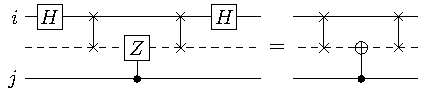
\includegraphics[width=0.8\textwidth]{customcnot.pdf}
\end{center}

Notar que el fonón, que actua colectivamente, nos permite acoplar
iones $i$ con iones $j$.

La puerta CNOT, junto a las puertas de un qubit, nos permite construir
cualquier circuito cuántico, de forma similar a como la puerta XOR en
circuitos clásicos permite simular cualquier circuito.

En la práctica, los fonones tienen tiempos de coherencia bajos, a
diferencia de los iones, y dificultan la construcción de estos
aparatos. Hay propuestas alternativas, basadas por ejemplo en
semiconductores.

\subsection{Cadena contínua de osciladores}
Es un problema interesante, ya que sirve como introducción a la teoría
cuántica de campos. El paso más grande conceptualmente es sustituir
$X_n$, con $n\in \mathbb{N}$, por $ξ(x)$. % <\endclass>

% New Notes: Fri Nov 11 12:16:25 CET 2016

\part{Mecánica cuántica relativista}

\chapter{Mecánica cuántica no relativista de Feynmann}

\section{Acción clásica}
La acción clásica se define como
\begin{equation}
  S = \int_{t_a}^{t_b} \mathcal{L} (\dot{x},x) \dd{t}
\end{equation}
quedando el sistema completamente descrito por $\dot{x}(t),x(t)$. Para
hallarlas, imponemos que
\begin{equation}
  \frac{δS}{δx}=\int_{t_a}^{t_b} \left( \pdv{L}{x}δx +
    \pdv{L}{\dot{x}} δ\dot{x} \right)=0
\end{equation}
Integrando por partes,
\begin{equation}
  \int_{t_a}^{t_b}  \left( \pdv{L}{x} - \dv{}{t} \pdv{L}{x} \right) δx \dd{t}
\end{equation}
Como tiene que ser cero para variaciones arbitrarias, $\left(
  \pdv{L}{x} - \dv{}{t} \pdv{L}{x} \right) = 0$, lo que nos da junto a
las condiciones de contorno iniciales las trayectorias del sistema en
el espacio de fases.

\section{Formulación de Feynmann}
Si bien es completamente equivalente a otras formulaciones, es
especialmente conveniente para realizar la segunda cuantificación.

Imaginemos un experimento de doble rendija. Tenemos un punto emisor en
$(x_a,t_a)$ que emite electrones. Vemos que al tapar una rendija todos
los puntos se acumulan en el detector final en una posición, y de
forma similar para la otra. Bajando la intensidad del haz de
electrones, podemos ver que a pesar de lanzar sólo un electrón, las
interferencias provocadas por no tapar ninguna rendija siguen
provocándose. \emph{El electrón interfiere consigo mismo, no con los demás.}

Conceptualmente, puedo añadir más paredes tras la doble rendija,
demostrando que \emph{el electrón sigue todas las trayectorias posibles.}

Vemos que si bien en mecánica clásica el electrón sigue una
trayectoria definida en el espacio de fases, en cuántica el electrón
sigue todas las trayectorias posibles entre dos puntos defidos.
Formalizamos esto definiendo un intervalo $t+\dd{t}$ y $x+\dd{x}$ y
calculando la probabilidad de que el electrón cruce ese punto, que no
es más que el módulo de la función de ondas $Ψ(x,t)$ al cuadrado.

Definimos el \emph{propagador de Feynmann} $k(\mathbf{b},\mathbf{a})$
como $\bra{x_b,t_b}\ket{x_a,t_a}$, la probabilidad de dicha
transición:
\begin{equation}
  k(\mathbf{b},\mathbf{a}) = \sum_{n} e^{-i \frac{t}{ℏ}(t_b-t_a)} φ_n(x_b)φ^*_n(x_a)
\end{equation}

Vemos por ejemplo que cuando $t_b-t_a \to \infty$, la función de ondas
acaba cayendo al estado fundamental, siendo la probabilidad de otros
estados nula.

Si tomamos un tiempo imaginario, $t/ℏ\simeq β$ y tenemos una conexión
con la mecánica estadística (aparece una suma de energías $e^{βE}$).

Hasta aquí, se tiene una formulación estándar de la mecánica cuántica.
El paso de Feynmann fue suponer que
\begin{equation}
  k(\mathbf{b},\mathbf{a}) = \sum_{\text{tray.}} e^{i S(x)/ ℏ}
\end{equation}
escribiendo el propagador como suma de trayectorias. El propagador
equivale a trabajar con ondas, mientras que la mecánica clásica es la
aproximación de esas ondas a rayos, de forma análoga a la óptica.

Vemos que en el límite en que $S(x)\gg ℏ$, cambiando
infinitesimalmente las trayectorias obtenemos grandes variaciones de
fase, cancelándose dicha contribución\footnote{De forma similar,
  $\sum_{α} e^{iα} \simeq 0$.}. Las únicas que no se cancelan
son las que cumplen que no varían, $ \frac{δS(x)}{δx}=0$, recuperando
para acciones grandes la mecánica clásica.

Para formalizar esta idea intuitiva, discretizamos las coordenadas
espaciales y temporales, $t_n = t_0 + n ε$ y $x(t_n) = x_n$, además de
$t_b-t_a=Nε$.
\marginnote{La generalización a más dimensiones es trivial. El
  lagrangiano se supone $\mathcal{L}= \frac{1}{2}m \dot{x}(t)^2 -V(x)$.}
Calculamos la acción:
\begin{equation}
  S = \int_{t_a}^{t_b}a \mathcal{L}(\dot{x},x) \dd{t}= ε\sum_{n}
  \left[ \frac{1}{2} m \left( \frac{x_{n+1}-x_n}{ε} \right)^2 -V(x_n)
  \right]
\end{equation}
El propagador será, tomando el límite $ε\to 0$,
\begin{equation}
  k(\mathbf{b},\mathbf{a}) =  \frac{1}{A} \int_{-\infty}^{\infty}
  \frac{\dd{x_1}}{A} \cdots \frac{\dd{x_{N-1}}}{A} e^{\frac{iε}{ℏ}
    \sum_{n=0}^{N-1} \left( \frac{1}{2}m \left( \frac{x_n-x_{n-1}}{ε} -V(x)??? \right)^2 \right)}
\end{equation}
de forma que
\begin{equation}
  k(\mathbf{b},\mathbf{a}) = \frac{1}{A} \int_{\mathbb{R}}
  \prod_{n=1}^{N-1} \frac{\dd{x_n}}{A}
e^{\frac{iε}{ℏ}
    \sum_{n=0}^{N-1} \left( \frac{1}{2}m \left( \frac{x_n-x_{n-1}}{ε} \right)^2  -V(x)\right)}
\end{equation}
con $A$ una constante que se escogerá para que estas cuentas tengan sentido.
Sabemos que $k(\mathbf{b},\mathbf{a})= \int_{\mathbb{R}}
k(\mathbf{b},\mathbf{c}) k(\mathbf{c},\mathbf{a}) \frac{\dd{x_c}}{A}$.
Introduciendo eso en la ecuación anterior,
\begin{equation}
  k(\mathbf{b},\mathbf{a}) = \int_{\mathbb{R}} \prod_{n=0}^{N-1}
  k(x_{n+1},x_n) \dd{x_n}
\end{equation}
y
\begin{equation*}
  k(x_{n+1},x_n) = \frac{1}{A} e^{\frac{iε}{ℏ} L \left[
      \frac{x_{n+1}-x_n}{ε},\ V(x_n) \right]}
\end{equation*}
\marginnote{Notar como hasta ahora no a aparecido ningún operador
  cuántico, y la formulación es completamente clásica.}

Para calcular $A$, consideramos una partícula libre\footnote{
  \begin{equation}
    \begin{split}
      \mathcal{L} &= \frac{1}{2} m \int_{t_a}^{t_b} \dot{x}(t)^2
      \dd{t} \\
      &\to \frac{εm}{2} \sum_{n=0}^{N-1} \left( \frac{x_n-x_{n+1}}{ε}
      \right)^2
    \end{split}
  \end{equation}
}.

\begin{equation}
  k(\mathbf{b},\mathbf{a}) = \frac{1}{2} \int_{-\infty}^{\infty}
  \prod_{n=0}^{N-1} \frac{\dd{x_n}}{A} e^{\frac{im}{2 ℏε}
    \sum_{n=0}^{N-1} (x_n - x_{n+1})}
\end{equation}
que es idéntico a
\begin{equation}
  k(\mathbf{b},\mathbf{a}) = \frac{1}{2} \int_{-\infty}^{\infty}
  \prod_{n=0}^{N-1} \frac{\dd{x_n}}{A} e^{\frac{im}{2 ℏε}
    \sum_{n=1}^{N} (-x_{n-1} + x_n)}
\end{equation}
\marginnote{
  \begin{align*}
    \int_{-\infty}^\infty e^{-λx^2+bx} \dd{x} &= \sqrt{\frac{π}{λ}}
                                                e^{\frac{b^2}{4λ}}\\
    \int_{-\infty}^\infty e^{i(λx^2+bx)} \dd{x} &= \sqrt{\frac{iπ}{λ}} e^{\frac{-ib^2}{4λ}}
  \end{align*}
}
Reescribimos la integral como
\begin{equation}
  \begin{split}
    I_G(A,B) &= \int_\mathbb{R} \prod_{n=1}^N \dd{x_n}
    e^{-\sum_{i,j=1}^N x_i A_{ij} x_j + \sum_{n=1}^N (B_n + B_n^*)x_n}\\
    &= \int_\mathbb{R} \dd{x_n}t e^{-(x|Ax)+(B|x)+(x|B)}
  \end{split}
\end{equation}
donde se han utilizado productos escalares . Obtenemos,
consultando tablas de integrales,
\begin{equation}
  I_G(A,B) = \frac{π^{N/2}}{(\det A)^\oh} e^{(B|A^{-1}B)}
\end{equation}

Por lo tanto, aplicando esto,
\begin{equation}
  \begin{split}
    k(\mathbf{b},\mathbf{a}) &= \left( \frac{1}{A} \right)^N
    \int_\mathbb{R} \prod_{n=1}^{N-1} \dd{x_n} e^{\frac{im}{2 ℏε}
      (x_0^2+x_N^2+2x_1^2 -x_0x_1-x_1x_2+2x_2^2+\cdots)} \\
    &= \left( \frac{1}{A} \right)^N \int_\mathbb{R} \prod_{n=1}^{N-1} \dd{x_n}
    e^{\frac{im}{2 ℏε}(x_0^2+x_n^2+(x|y) + (y|x) + (x|Bx))}
  \end{split}
\end{equation}
donde se ha desarrollado el sumatorio.
\marginnote{$x=(x_1, x_2,\cdots,x_{N-1})^T$ y
  $y=(x_0,0,0,\cdots,0,x_N)^T$. La matriz $B$ será
  \[
    B = \mqty(
    2 & -1 & 0 &0 & \cdots & 0 \\
    -1 & 2 & -1 &0&  \cdots & 0 \\
    0 & -1 & 2 &-1&  \cdots & 0 \\
    \vdots & \vdots & \vdots &\vdots&  \ddots & \vdots \\
    0 & 0 & 0 & \cdots & -1 & 2
    )
  \]
}
\begin{equation}
  k(\mathbf{b},\mathbf{a}) = \left( \frac{1}{A} \right)^N
  \frac{π^{\frac{N-1}{2}}}{(\det B)^\oh} \frac{1}{ \left( \frac{im}{2
        ℏε} \right)^{\frac{N-1}{2}}} e^{\frac{im}{2 ℏε} (x_0^2 + x_N^2
    - (y|B^{-1}y))}
\end{equation}
Necesitamos calcular el determinante de $B$, que no es más
que $\det B = \prod_{n=1}^{N-1} \frac{n+1}{n} = N$ tras diagonalizar
la matriz. Para $(y|B^{-1}y)$ puede parecer que hay que invertir $B$,
pero recordando la forma de $y$ sólo necesitamos unos cuantos
elementos. \emph{At the end of the day}, obtenemos
\begin{equation}
  k(\mathbf{b},\mathbf{a}) = \left( \frac{1}{A} \right)^{N} \left(
    \frac{2πi ℏε}{m} \right)^{\frac{N-1}{2}} \frac{1}{N^\oh}
  e^{\frac{im}{2 ℏ} \frac{(x_b-x_a)^2}{Nε = t_b-t_a}}
\end{equation}
Esta expresión es conocida en mecánica cuántica, y tiene valor
\begin{equation}
\int
e^{-i \frac{E_k(t_b-t_a)}{ℏ}} φ^*(x_a)φ(x_b) = \left( \frac{m}{2πi
    ℏ(t_b-t_a)} \right)^\oh e^{\frac{im}{2 ℏ} \frac{(x_b-x_a)^2}{t_b-t_a}}
\end{equation}
\marginnote{
  \begin{align*}
    φ(x) &= \frac{1}{\sqrt{2π}} e^{ikx} \\
    E_k &= \frac{ℏ^2}{2m} k^2
  \end{align*}
}
Para que coincidan, necesitamos
\begin{equation}
  \boxed{
    A = \left( \frac{2π i ℏ ε }{m} \right)^\oh
  }
\end{equation}

Con ella, se tiene definido el propagador y como calcularlo, todo con
mecánica clásica. A continuación, veamos si se puede recuperar la
ecuación de Schrödinger.

\begin{itemize}
\item $Ψ$ es la probabilidad de que la partícula esté en un punto del
  espacio de fases.
\item $k(\mathbf{b},\mathbf{a})$ es la probabilidad de que esté en un
  punto \emph{viniendo de otro}.
\end{itemize}

Por tanto,
\begin{equation}
  Ψ(x, t) = \int k(x,t;\ x_a,t_a) Ψ(x_a,t_a) \dd{x_a}
  \label{eq:matame}
\end{equation}

de forma que la función de ondas está relacionada con el propagador de
Feynmann. Escribamos \eqref{eq:matame} en un intervalo de tiempo
corto:
\begin{equation}
  \begin{split}
    Ψ(x, t+\dd{t}) &= \int \frac{\dd{y}}{A} e^{\frac{iε}{ℏ} \left[
        \frac{1}{2} m \left( \frac{x-y}{ε} \right)^2 - V(x) \right]}
    \\
    &= Ψ(x,t) - \frac{iε}{ℏ} V(x) Ψ(x,t) + \frac{1}{2}
    \dv[2]{Ψ(x,t)}{x} \int η^2 e^{\frac{im}{2 ℏε}η^2} \frac{\dd{η}}{A}
    + \cdots
  \end{split}
\end{equation}
desarrolando en serie de Taylor $Ψ(x+η,t)$.

Obtenemos
\begin{equation}
  i ℏ \left( \frac{Ψ(x,t+\dd{t}) - Ψ(x, t)}{ε} \right) = \frac{-1}{2m}
  \dv[2]{}{x} Ψ(x,t) + V(x) Ψ(x, t) + \order{ε}
\end{equation}
Tomando $ε\to 0$, recuperamos $i ℏ \pdv{}{t} Ψ(x,t) = \Ham Ψ(x,t)$.

% New Notes: Tue Nov 15 12:09:42 CET 2016

\section{Oscilador armónico}
Antes de resolverlo, veamos una propiedad especial de la acción. Sea
un lagrangiano $\mathcal{L}= a_0 \dot{x}(t)^2 + a_1 x(t)\dot{x}(t) +
a_2 x(t)^2 + a_3 x(t) + a_4$. Tiene todos los términos hasta orden
$\order{x^2}$ excepto el de $\dot{x}$, pero este no es necesario, ya
que $\int_{t_a}^{t_b} a_5 \dot{x}(t) \dd{t}$ se puede escribir
integrando por partes como $\int_{t_a}^{t_b} \dv{a_5(t)}{t} x(t)
\dd{t} + \eval{a_5(t)x(t)}_{t_a}^{t_b}$. El primer término lo podemos
meter con los demás, y el segundo se elimina sin más que mover el
origen de las acciones.

La acción clásica nos dara una $\bar{x}$ tal que
\begin{equation}
  \eval{\dv{}{t} \pdv{S}{\dot{x}}}_{x=\bar{x}} = \eval{\frac{δS}{δx}}_{x=\bar{x}}
\end{equation}
Escribo mi trayectoria como la clásica, $\bar{x}(t)$, más una
desviación $y(t)$:
\begin{align}
x(t) = \bar{x}(t) + y(t)
\dot{x}(t) = \bar{\dot{x}}(t) + \dot{y}(t)
\end{align}
donde $\bar{x}(t_a)=x_a \rightarrow y(t_a)=0$ e igual para $t_b$.

Sustituyendo en el lagrangiano, obtendré el lagrangiano clásico
$\mathcal{L}(\bar{\dot{x}},\bar{x})$ más términos extra.

Empleando el resultado del ejercicio 1.2\footnote{
  % Ej. 1.2
  % S[x] puede escribirse como S[xclásica] + ∫t_a -> t_b  (a0 doty^2) ...
  \begin{equation*}
    \begin{split}
    \mathcal{S}[x] &= \mathcal{S}[\bar{x}] +\\ &\int_{t_a}^{t_b} (a_0
    \dot{y}^2 +a_1 y \dot{y} + a_2 y^2 + a_3 y + a_4) \dd{t}
    \end{split}
  \end{equation*}
}, notamos que es equivalente a $\mathcal{S}[x] = \mathcal{S}[\bar{\dot{x}},\bar{x}]
+ \mathcal{S}[{\dot{y}},{y}]$, y por tanto
\begin{equation}
  \begin{split}
    k(\mathbf{b},a) &= \int_{x(t_a)=x_a}^{x(t_b)=x_b} [\dd{x}]
    e^{i\mathcal{S}/ ℏ} = e^{i\mathcal{S}[\bar{\dot{x}},\bar{x}]/ ℏ}
    \int_{y(t_a)=0}^{y(t_b)=0} [\dd{y}] e^{i \mathcal{S}(\dot{y},y)/
      ℏ} \\ &= e^{i \mathcal{S} [\bar{\dot{x}},\bar{x}]/ ℏ} F(t_b,t_a)
  \end{split}
\end{equation}

de forma que $F(t_b,t_a) = \frac{1}{A} \int \prod \frac{\dd{y_n}}{A}
e^{i \frac{ε}{ℏ}\sum \mathcal{S}(y_n,y_{n+1})}$.

Utilizamos esto con el lagrangiano de un oscilador armónico,
$\mathcal{L}= \frac{1}{2} m \dot{x}(t)^2 - \frac{1}{2} m ω^2 x(t)^2$.
La ecuación del movimiento es
\begin{equation}
  m ω^2 x(t) = - m \ddot{x}(t)
\end{equation}
con las condiciones de contorno $x(t_a)=x_a$ y $x(t_b)=x_b$, de forma
que
\begin{equation}
  \bar{x}(t) = x_a \cos ( ω(t-t_a)) + c \sin(ω(t-t_a))
\end{equation}

% This is other ej.
La acción clásica es expresable como
\begin{equation}
  \mathcal{S} [\bar{x}] = \frac{mω}{2\sin(ωT)} [ (x_a+x_b)^2 \cos(ωT)-2x_ax_b]
\end{equation}
con $T=t_b-t_a$.

Calculamos $F(T)$,
\begin{equation}
  F(T) = \left( \frac{1}{A} \right)^N \int \prod_{n=1}^{N-1} \dd{y_n}
  e^{\frac{im}{2 ℏε} \sum_{n=1}^N [ (y_n -y_{n-1})^2 - mω^2 ε^2 y_n^2]}
\end{equation}

% Interludio

% Other ej. λ_k one

Los cálculos son similares a la última vez (partícula libre); llegamos
a
\begin{equation}
  F(T) = \left( \frac{mω}{2πi ℏ\sin(ωT)} \right)^\oh
\end{equation}
con propagador
\begin{equation}
  k(\mathbf{x}_b,t_b; \mathbf{x}_a,t_a) = \left( \frac{mω}{2π i ℏ
      \sin(ωT)} \right)^\oh e^{ \frac{imω}{2 ℏ \sin(ωT)}[ (x_a^2+x_b^2
    \cos(ωT))-2x_ax_b]}
\end{equation}
que ha de ser igual a
\begin{equation}
  \sum_{n} e^{-i(n+\oh) T/ ℏ} ϕ^*_n(x_a) ϕ_n(x_n)
\end{equation}

Si estamos en un número superior de dimensiones ($N$), el propagador será
\begin{equation}
  k(\mathbf{b},\mathbf{a}) = \left( \frac{1}{A} \right)^{3N} \int [\dd{\mathbf{x}}]
    e^{i \mathcal{S}[ \dot{\mathbf{x}},\mathbf{x}]/ ℏ}
\end{equation}

Por ejemplo, para el caso libre se obtiene
\begin{equation}
  k(\mathbf{x}_b, t_b; \mathbf{x}_a,t_a) = \left( \frac{1}{A}
  \right)^{3N} \int \prod_{k=1}^{N-1} \dd{x_n} \dd{y}_k \dd{z}_k
  e^{\frac{iε}{ℏ} \sum_{n=1}^N \left[ \left( \frac{x_n-x_{n-1}}{ε}
      \right)^2
      + \left( \frac{y_n-y_{n-1}}{ε} \right)^2
      +  \left( \frac{y_n-y_{n-1}}{ε} \right)^2
    \right]}
\end{equation}
Vemos que al tener un lagrangiano separable, el propagador es
escribible como producto de propagadores.


\chapter{Breve repaso de la relatividad especial}

\section{Notación}

Comencemos por introducir la notación más usual en teoría cuántica de
campos. Tendremos vectores contravariantes
$x^\mu=(ct,x,y,z)=(ct,\mathbf{x})$
\marginnote{
  Los índices griegos varían en $\{0,1,2,3\}$ y los latinos
  en $\{1,2,3\}$. Los latinos expresan coordenadas espaciales, y la
  componente $0$ expresa el tiempo.
}.
Los tensores contravariantes se transforman\footnote{
  Se supone la velocidad en el eje $\hat{x}$. Si no, basta con rotar
  el sistema de referencia.
} según
\begin{align}
  ct' &= \frac{ct-βx}{\sqrt{1-β^2}} \\
  x' &= \frac{x - βct}{\sqrt{1-β^2}} \\
  y' &= y \\
  z' &= z
\end{align}
con $β=v/c$. De forma más compacta,
\begin{equation}
  x'^{1} = γ(x^1-βx^0)
\end{equation}
y $x^2,x^3$ se mantienen constantes.

A cualquier vector de cuatro componentes que cumpla estas
transformaciones, se le denotará \emph{cuadrivector bajo el
  grupo de Lorentz}. Veremos que, por ejemplo, $A^μ=(ϕ,\mathbf{A})$ o
$J^μ=(cρ,\mathbf{J})$, o $p^μ=(\frac{E}{c},\mathbf{p})$ lo son.

Los vectores covariantes se definen como
\begin{equation}
  x_μ = g_{μν} x^η
\end{equation}
con
\begin{equation}
g_{μν}= \mqty(1&0&0&0 \\ 0 & -1 &0 & 0 \\ 0 &0 &-1 & 0 \\0 & 0 &0
& -1 )
\end{equation}
donde se emplea el convenio de Einstein, y se sobreentiende un
sumatorio sobre índices repetidos.

Notamos que $x^μx_μ= c^2t^2 - \mathbf{x}^2$ es un invariante, y que el
tensor métrico $g_{μν}$ es el que nos permite subir y bajar
índices\footnote{
  Subir y bajar índices temporales no cambia el signo, pero sí bajar y
  subir índices espaciales.
}.

Tratamos de escribir las ecuaciones de Lorentz con un tensor $Λ\indices{_ν^μ}$,
de forma que $x'^μ = Λ\indices{_ν^μ} x^ν$. Obtenemos
\begin{equation}
Λ\indices{_ν^μ} = \mqty(
γ & -βγ  & 0 & 0 \\
-βγ & γ & 0  & 0 \\
0 & 0 & 1& 0 \\
0 & 0 & 0& 1 \\
)
\end{equation}
con $γ = \frac{1}{\sqrt{1-β^2}}$. Puede comprobase que $x_μ' = Λ\indices{_μ^η}
x_η$, donde
\begin{equation}
  Λ\indices{_μ^ν} = \mqty(
γ & +βγ  & 0 & 0 \\
+βγ & γ & 0  & 0 \\
0 & 0 & 1& 0 \\
0 & 0 & 0& 1 \\
  )
\end{equation}
y $Λ\indices{_μ^ν} Λ\indices{_ν^μ} = \mathbb{I}$.
Para describir estas
transformaciones como rotaciones en el grupo de Lorentz, se define
$\tanh(ω)=β$ de forma que $\cosh ω = γ$. En tal caso,
\begin{equation}
Λ\indices{_ν^μ} = \mqty(
\cosh ω  & -\sinh ω & 0 & 0 \\
-\sinh ω & \cosh ω  & 0 & 0 \\
0        & 0        & 1 & 0 \\
0        & 0        & 0 & 1 \\
)
\end{equation}

Definiremos producto escalar\footnote{A pesar de no ser definido
  positivo.} de un vector consigo mismo como $x^μ g_{μν}x^ν$, de forma
que obtengamos el invariante $(ct)^2-\mathbf{x}^2$.
Notamos que si $x^μ=(ct,\mathbf{x})$, se tiene
\begin{align}
  x_μ = g_{μν}x^ν=(ct,-\mathbf{x})
\end{align}

Vemos que, en efecto, $x'^μ x'_μ = Λ\indices{^μ_ν} x^ν Λ\indices{_μ^σ} x_σ = x^ν x_σ δ^{σ,ν} = x^ν x_ν$.

Notando que esto sólo es un caso particular (movimientos en
$\hat{x}$), nos preguntamos por el caso general; simplemente hay que
rotar el tensor métrico y las $Λ$, que adquieren una expresión
matricial mucho más complicadas. En lo que sigue, nos limitaremos a
rotar los sistemas de forma que podamos emplear las expresiones
anteriores.

Definimos el elemento diferencial de tiempo propio, $\dd{τ}$, como
$ \frac{1}{c}\sqrt{\dd{x^μ}\dd{x_μ}}=\dd{t}\sqrt{1-β^2} = \dd{t}
γ^{-1}$. Notamos que es invariante.

Las velocidades se definen como $u^i = \dv{x^i}{t} = c \dv{x^i}{x^0}$.
Con esta definición, podemos ver como se transforman sus componentes.
En general, nos fijamos en como se transforman las derivadas, nos
fijamos en que $x^μx_μ$ es invariante e igual a $x^μ g_{μν}x^ν$.
Derivamos dicha expresión frente a $x^σ$, $\pdv{x^σ} (x^μx_μ)$:
\begin{equation}
  \pdv{x^σ} x^μ x_μ = \pdv{x^σ} x^μ x_μ g_{μν} = x^ν g_{μν} δ_σ^μ +
  x^μ g_{μν} δ_{σ}^ν = x_σ + x_σ = 2x_σ
\end{equation}
Vemos que se transforma como un vector covariante.
\marginnote{Obtenemos $1$ cuando $σ=ν$ o el indice correspondiente por
  la misma razón que $\dv{x}{x}=1$ y $\dv{x}{y}$ = 0}.

\section{Potencial y tensor electromagnético}
Recordamos las ecuaciones\footnotemark de Maxwell,
\begin{center}
  \begin{tabular}{cc}
    $\displaystyle \nabla \mathbf{B}=0$
    &
      $\displaystyle \nabla \mathbf{B}- \frac{1}{c} \pdv{t} \mathbf{E} = \frac{4π}{c}\mathbf{J}$
    \\
      $\displaystyle \nabla \mathbf{E}=4πρ$
    &
    $\displaystyle \nabla \times \mathbf{E} +\frac{1}{c} \pdv{t} \mathbf{B}=0$
    \\
  \end{tabular}
\end{center}
\footnotetext{En ocasiones se emplearán unidades de Gauss para aliviar
las ecuaciones.}

Introducimos un campo electromagnético $A^μ = (ϕ,\mathbf{A})$, de
forma que $\mathbf{B}=\nabla \times \mathbf{A}$ y $\mathbf{E} = -
\nabla A^0 - \frac{1}{c} \pdv{t} \mathbf{A}$. $ϕ$ es el potencial
escalar usual. Inmediatamente,
\begin{align}
  \nabla \mathbf{B} &= \nabla(\nabla \times \mathbf{A}) = 0 \\
  \nabla \times \mathbf{E} + \frac{1}{c} \pdv{t} \mathbf{B}
                    &= -\nabla \times (\nabla A^0) - \frac{1}{c}
                      \nabla \pdv{t} \mathbf{A} + \frac{1}{c} \pdv{t}
                      \mathbf{B} = \cdots = 0
\end{align}

De forma que se cumplen ya dos de las ecuaciones de Maxwell. Para las
otras dos, definimos el \emph{tensor electromagnético}:
\begin{equation}
  F^{μν} = \partial^μ A^ν - \partial^ν A^μ = - F^{νμ}
\end{equation}
Al ser un tensor antisimétrico, la diagonal está llena de ceros. En el
resto de los componentes, se tiene
\begin{align}
 F^{0i} &= -E^i \\
  F^{jk} &= - \epsilon^{jkl}B^l
\end{align}
En forma matricial,
\begin{equation}
  F^{μν} = \mqty(
  0 & -E^1 & -E^2 & -E^3\\
  E^1 & 0 & -B^3 & -B^2 \\
  E^2 & B^3 & 0 & -B^1 \\
  E^3 & -B^2 & B^1 & 0
  )
\end{equation}
y para $F_{μν}$,
\begin{equation}
  F_{μν} = \mqty(
  0 & E^1 & E^2 & E^3\\
  -E^1 & 0 & -B^3 & -B^2 \\
  -E^2 & B^3 & 0 & B^1 \\
  -E^3 & -B^2 & B^1 & 0
  )
\end{equation}
\marginnote{Se emplea $J^μ = (cρ,\mathbf{J})$}
Con él, podemos ver como en $\partial_μ F^{μν} = \frac{4π}{c}J^ν$
están las dos ecuaciones de Maxwell restantes. Con $ν=0$ recuperamos
$\nabla \mathbf{E} = 4πρ$, y con $ν$ distinto de cero, recuperamos
$\nabla \mathbf{B}- \frac{1}{c} \pdv{t} \mathbf{E} = \frac{4π}{c}
\mathbf{J}$.

Por lo tanto, sustituimos las ecuaciones de Maxwell por
\begin{equation}
  \boxed{
  \partial_μ F^{μν} = \frac{4π}{c} J^ν
  }
\end{equation}
definiendo $\mathbf{B} = \nabla \mathbf{A}$ y $\mathbf{E}= -\nabla A^0
- \frac{1}{c} \pdv{t} \mathbf{A}$.


Por su utilidad posterior, definimos un escalar, la \emph{densidad
lagrangiana}; es el equivalente del lagrangiano en campos:
\begin{equation}
  \mathbb{L} = \frac{-1}{16π} F_{μν}F^{μν} = \frac{1}{8π} (\mathbf{E}^2-\mathbf{B}^2)
\end{equation}
También se define el análogo al hamiltoniano, que en mecánica clásica
sólo tiene un componente, el \emph{tensor energía-impulso}:
\begin{equation}
  T^{μν} =  \sum_{α} \frac{δ \mathbb{L}}{δ (\partial_μ
    A_α)} \partial^ν A_α - g^{μν} \mathbb{L}
\end{equation}
Su componente $T^{00} = \frac{1}{8π}(\mathbf{E}^2+\mathbf{B}^2) +
\frac{1}{4π} (\mathbf{E}\nabla A^0)$ es la densidad de energía del
campo electromagnético.


\subsection{Invariancia Gauge}
Imaginemos un campo electromagnético $A'^μ = A^μ + \partial^μ Λ$.
Entonces,
\begin{align}
  A'^0 &= A^0 + \partial^0 Λ \\
  \mathbf{A}' &= \mathbf{A} + \nabla Λ
\end{align}
Obtenemos que $\mathbf{B}' = \nabla \mathbf{A}' = \nabla \mathbf{A} =
\mathbf{B}$, y de forma similar para el campo eléctrico obtenemos
$\mathbf{E}' = - \nabla A^0 - \frac{1}{c} \pdv{t} \mathbf{A}' = \cdots
=\mathbf{E}$.
De forma más elaborada, también se concluye que $F'^{μν}=F^{μν}$.

Concluimos que hay varios campos electromagnéticos que nos dan el
mismo campo $\mathbf{E}$ y $\mathbf{B}$. Esto nos permite tener unos
grados de libertad extra, que se fijarán en función de lo que más
convenga para el problema a tratar.

A simplificar los campos explotando esta propiedad se le llama
\emph{transformación gauge}. Entre las más usadas, está el \emph{gauge
de Coulomb}, que tiene dos versiones:
\begin{itemize}
\item En presencia de cargas eléctricas, se suele fijar $\nabla
\mathbf{A}'=0$, también llamado \emph{gauge
  transversal}. Para ello, se escoge
\begin{equation}
  Λ(\mathbf{r}) = \frac{1}{4π} \int
  \frac{\dd{\mathbf{r}'}}{\abs{\mathbf{r}-\mathbf{r}'}} \nabla
  \mathbf{A}(\mathbf{r},t)
\end{equation}
Sin cargas, $A'^0$ se puede tomar nulo.
\item En ausencia de cargas electricas, fijamos $A'^0=0$; se suele
  denotar a este gauge \emph{gauge de radiación}. Para ello, empleamos
  \begin{equation}
    Λ'(\mathbf{r}) = -c \int_{t_0}^t A^0 \dd{t'}
  \end{equation}
  con $t_0$ un valor arbitrario de $t$, por ejemplo cero.
\end{itemize}

Uno de los inconvenientes que tiene el gauge de Coulomb es que no es
covariante. Por ello, a veces se emplea el \emph{gauge de Lorentz},
definido como
\begin{equation}
  \partial_μ A^μ = 0
\end{equation}
que es invariante Lorentz.


\chapter{La ecuación de Klein-Gordon}
Partimos de $E=\sqrt{\mathbf{p}^2c^2 + m^2c^4}$, y empleando $E= i
ℏ \partial_t$ y $ \mathbf{p}= i ℏ \nabla$
, obtenemos la \emph{ecuación de Schrödinger no relativista},
\begin{equation}
  i ℏ\partial_t Ψ = \sqrt{- ℏ^2 c^2 \nabla^2 + m^2 c^4} ⋅ Ψ
\end{equation}

Se abandonó rápidamente por ser no local y complicada de manejar.
Se quiere una ecuación de primer orden en la derivada respecto del
tiempo, de forma que baste con dar $Ψ(t_0)$ como condición de
contorno. Como no se puede obtener esto, nos conformamos con una
ecuación de segundo orden; empleando $E^2$ en lugar de $E$, para
eliminar la raíz, obtenemos
\begin{equation}
  - ℏ^2 \pdv[2]{t} Ψ =(- ℏ^2 c^2 \nabla^2 + m^2c^4) Ψ
\end{equation}
Dividiendo entre $c^2$, se puede escribir como
\begin{equation}
  \left(\dalambert + \frac{m^2 c^2}{ℏ^2}\right) Ψ = 0
\end{equation}
con $\dalambert = \partial_μ\partial^μ$ el \emph{D'Alambertiano}.

Resolver esta ecuación es trivial, ya que se conocen los autoestados
de $\nabla$; tomando $Ψ= \frac{1}{(2π)^4} e^{iP_μ x^μ / ℏ}$ nos queda
$p_0^2 = \frac{E^2}{c^2} =\mathbf{p}^2+m^2c^2$, obteniendo el
resultado esperado ($\abs{E} = \sqrt{p^2c^2 + m^2c^4}$). Notamos que
$E = \pm\sqrt{p^2c^2 + m^2c^4}$, de forma que nos aparece un signo
nuevo.

$E$ no está acotada inferiormente, lo que nos imposibilita tener un
estado fundamental y un origen de energías. No obstante, se empleará
este resultado, hasta que se realice una segunda cuantificación y se
introduzca la antimateria.

Notamos también que $\int ρ \dd[3]{x}=1$, pero el volumen
\marginnote{$ρ$ denota la densidad de probabilidad.}
cambia al realizar transformaciones de Lorentz. Por ello, para
mantener la igualdad, $ρ$ no puede ser simplemente $Ψ^*Ψ$, que es
invariante.

Restando $Ψ(\dalambert + \frac{m^2c^2}{ℏ^4})Ψ^*=0$ a su ecuación
conjugada, obtenemos $\partial_μ (Ψ^* \partial^μ Ψ - Ψ \partial^μ
Ψ^*)=0$, y podemos definir la corriente de probabilidad como
\begin{equation}
  J^μ = \frac{i ℏ}{2m}(Ψ^* \partial^μ Ψ - Ψ \partial^μ Ψ^*)
\end{equation}
de forma que tenemos una \emph{cuadricorriente} que se conserva
($\partial_μ J^μ = 0$).
\marginnote{
  De nuevo, se tiene $J^μ = (cρ,\mathbf{J})$, con
  \begin{align}
    ρ &= \frac{i ℏ}{2mc} (Ψ^* \partial^0 Ψ -
    Ψ \partial^0 Ψ^*)\\
    \mathbf{J} &= \frac{-i ℏ}{2mc} (Ψ^* \nabla Ψ -
    Ψ \nabla Ψ^*)
  \end{align}
}

Notamos que $\pdv{t} \int \dd[3]{x} ρ =0$, como se esperaba (la
probabilidad se conserva). No obstante, $ρ$ no es definida
positiva, así que no se puede interpretar rigurosamente como una
densidad de probabilidad. Esto se arregla introduciendo la antimateria
en la segunda cuantización.

Notando que hasta ahora todas las partículas eran libres, introducimos
un campo electromagnético.

\section{Interacción con un campo EM}
Cambiamos $p^μ= i ℏ \partial^μ$ por $p^μ - \frac{e}{c}A^μ$ en
$(\partial_μ \partial^μ + \frac{m^2 c^2}{ℏ^2})Ψ =0$, de forma que
obtenemos

\begin{equation}
  \frac{1}{c^2}\left( i ℏ\partial_t - \frac{e}{c}A_0 \right) \left( i ℏ\partial_t -
  \frac{e}{c_0} \right) Ψ = \left[ (i ℏ\nabla + \frac{e}{c} \mathbf{A})^2 +
    m^2c^2 \right] Ψ
\end{equation}

En el límite no relativista podemos escribir $Ψ = e^{-imc^2t/ ℏ} φ$, y
al introducirlo en la ecuación (despreciando la energía
electrostática, entre otras aproximaciones) obtenemos
\begin{equation}
  \left[ 2m(i ℏ \partial_t - eA_0) - \frac{i ℏe}{c} \pdv{A_0}{t}
  \right] Ψ = \left( i ℏ\nabla + \frac{e}{c} \mathbf{A} \right)^2 Ψ
\end{equation}

Si $\pdv{A_0}{t} = 0$,
\begin{equation}
  i ℏ\partial_t Ψ = \left( \frac{-ℏ^2}{2m} \nabla^2 + \frac{i ℏ}{mc}
    \mathbf{A} \nabla + \frac{ie ℏ}{2mc} \partial_μ A^μ + e A_0
  \right) Ψ
\end{equation}
y volviendo a escribir $Ψ = e^{-imc^2t/ ℏ} φ$ y realizando las
aproximaciones pertinentes,
\begin{equation}
  i ℏ\partial_t φ = \left(  \frac{-ℏ^2}{2m}\nabla^2 + eA_0 + \frac{i
      ℏ}{me} \mathbf{A} \nabla + \frac{ie ℏ}{2mc} \partial_μ A^μ
  \right) φ
\end{equation}
En el gauge de Coulomb, el sumando $\partial_μ A^μ$ se anula. La
ecuación es análoga a la que obtendríamos añadiendo a $i ℏ \partial_t$ el
término $eA_0$ en la ecuación de Schrödinger.

Para la ``densidad de probabilidad'', más bien interpretable como una
densidad de carga, se obtiene
\begin{equation}
  ρ = \frac{i ℏe}{2m} \left[ Ψ^* \partial_t Ψ - Ψ \partial_t Ψ^* +
    \frac{2ie}{ℏc^2} A^0 Ψ^*Ψ \right]
\end{equation}

Vemos que es similar a la densidad de probabilidad típica multiplicada
por la carga, pero queda también multiplicada por el potencial. Esto
hace que pueda cambiar de signo en algunas regiones, lo que puede
resultar molesto.

% New Notes: Fri Dec  2 12:13:25 CET 2016

\section{Ecuación de Klein-Gordon como sistema de ecuaciones}
Notando que la ecuación de Klein-Gordon \[\frac{1}{c^2}(i ℏ \partial_t
- eA_0)Ψ = \left[ (i ℏ \nabla + \frac{e}{c} \mathbf{A})^2 + m^2c^2
\right]Ψ\] es una ecuación de segundo orden, la escribimos como dos
ecuaciones de primer orden. Definimos
\begin{align}
  φ &= \frac{1}{2} \left[ 1 + \frac{i ℏ\partial_t - eA_0}{mc^2} \right] Ψ\\
  χ &= \frac{1}{2} \left[ 1 - \frac{i ℏ\partial_t - eA_0}{mc^2} \right] Ψ
\end{align}
y obtenemos
\begin{equation}
  i ℏ\partial_t Ψ = i ℏ\partial_t \mqty(φ\\ χ) = H_L Ψ
\end{equation}
donde
\begin{equation}
  H_L = e A_0 \mathbb{I} + i σ_2 \frac{(i h \nabla +
    \frac{e}{c}A)^2}{2m} + σ_3 \left[ \frac{(i ℏ\nabla +
      \frac{e}{c}A)^2}{2m} + mc^2 \right]
\end{equation}
y $σ_i$ son las matrices de Pauli. Al ser $H_L^2 = \left[ (m^2c^4 ) + c^2
  (i ℏ\nabla + \frac{e}{c}A)^2\right]\mathbb{I}$, ambas componentes de
$Ψ$ cumplen la ecuación de Klein-Gordon por separado.

Obtenemos una densidad de carga
\begin{equation}
  ρ = e (φ^*φ-χ^*χ)
\end{equation}
Vemos que una componente va de acuerdo con la carga, mientras que la
otra al reves. Empezamos a obtener resultados que nos recuerdan a
partículas y antipartículas.

Si empleamos una partícula libre $Ψ = \mqty(a\\ b) e^{-i(Et
  -\mathbf{p}\mathbf{x})/ℏ}$, obtenemos que $E^2 = p^2c^2 +m^2c^4$,
con autofunciones para $E>0$
\begin{equation}
  Ψ^+_\mathbf{p} = \mqty(a^+ \\ b^+) e^{-i P_μ x^μ / ℏ} = \mqty(a^+ \\ b^+)
  e^{-i(Et - \mathbf{p}\mathbf{x})/ℏ}
\end{equation}
con $a^+,b^+$ constantes. Para $E<0$,
\begin{equation}
  Ψ^-_\mathbf{p} = \mqty(a^+ \\ b^+) e^{+i(Et - \mathbf{p}\mathbf{x})/ℏ}
\end{equation}
donde se ha empleado que $E(\mathbf{p}) = E(-\mathbf{p})$ y se ha
cambiado el signo al momento ($Ψ^-_\mathbf{p}$ es en realidad
$Ψ^-_{-\mathbf{p}}$) para obtener
un invariante relativista en el paréntesis. En el límite no
relativista ($E\simeq mc^2$) se obtiene
\begin{align}
  Ψ^+_\mathbf{p} &= \frac{1}{\sqrt{V}} \mqty(1 \\ 0) e^{-iP_μ x^μ / ℏ}\\
  Ψ^-_\mathbf{p} &= \frac{1}{\sqrt{V}} \mqty(0 \\ 1) e^{+iP_μ x^μ / ℏ}
\end{align}

vemos que la componente superior corresponde a la partícula no
relativista moviéndose con momento $p$ y las de abajo corresponen a
una partícula similar de energía negativa y momento $-\mathbf{p}$. De
nuevo, las ecuaciones señalan la existencia de antimateria.

Notamos que si en la ecuación de Klein-Gordon,
\begin{itemize}
\item Cambiamos la carga $e$ por $-e$,
\item el momento $i ℏ\nabla$ por $- i ℏ\nabla$,
\item la energía $E$ por $-E$, o $Ψ$ por $Ψ^*$.
\end{itemize}
la ecuación es idéntica.


\chapter{La ecuación de Dirac}
En la teoría de la relatividad el tiempo es una coordenada más, y al
mezclar las transformaciones de Lorentz todas las coordenadas
se tiene que forzar una ecuación de primer orden en $t$, como se
deseaba, implica forzar también que sea de primer orden en las
coordenadas espaciales.

Partamos de una ecuación
\begin{equation}
i ℏ \partial_t Ψ= \left( -i ℏ
  \sum_{i=1}^3 α^i \partial_i + β mc \right)Ψ
\end{equation}
donde los coeficientes matriciales $α^j,β$ están por determinar.
Con ella, tomando una onda plana $Ψ(x) = N
e^{i(\mathbf{p}\mathbf{x}-Et)/ℏ}$, se obtiene
\begin{equation}
\frac{E}{c}
= \sum_{i=1}^3 α^i \mathbf{p}_i + β mc
\end{equation}
y elevando al cuadrado ambos lados de la ecuación,
\begin{equation}
  E^2 = c^2 \left( \sum_{ij}(α^iα^j)\mathbf{p}_i \mathbf{p}_j + c^3p \sum (α_i β + βα_i) +
    β^2 m^2 c^4 \right)
\end{equation}

Obtenemos una relación energía-momento, por lo que se ha de cumplir
\begin{align}
  α_iβ +β α_i &= 0 \\
  \frac{1}{2} (α^iα^j + α^jα^i) &= δ_i^j \\
  β^2 &= \mathbb{I}
\end{align}
\marginnote{Definimos el anticonmutador $\{A,B\}=AB+BA$.}
Además, $(α^i)^2 = \mathbb{I}$. La traza de $α^i$ será obviamente
igual a la traza de $α^iβ^2$ por ser $β^2=\mathbb{I}$, luego
\begin{equation}
  \tr α^i = \tr α^i β β = - \tr β α^i β = - \tr β^2 α^i = - \tr α^i
\end{equation}
De forma que $\tr α^i = 0$. De forma similar, $\tr β = 0$. Como $\Ham$
ha de ser autoadjunto, $α^j,β$ deberán ser hermíticas, y debido a que
$(α^j)^2=β^2=1$ sus valores propios serán $\pm 1$.

Concluímos,
\begin{itemize}
\item Las matrices $α,β$ han de tener dimensión par para tener tantos
  valores propios $+1$ como valores propios $-1$.
\item Podrían tener dimensión dos, pero eso requeriría cuatro matrices
  y sólo hay tres matrices de Pauli (que anticonmutan como
  requerimos)\footnote{En una dimensión sí que es posible emplearlas, ya
    que sólo se necesitamos 3.}. No nos queda más remedio que emplear
  matrices $4\times 4$.
\end{itemize}
Se suele emplear
\begin{align}
  α^i &= \mqty(0 && σ^i \\ σ^i && 0) \\
  β &= \mqty(\mathbb{I} && 0 \\ 0 && -\mathbb{I})
\end{align}
con $σ^i$ las matrices de Pauli.

Se define $γ = (β,α^i)$ por comodidad, de forma que la
ecuación quede como $(i ℏγ^μ \partial_μ-mc)Ψ = 0$. Empleando el
convenio de Feynmann, que define para todo operador $a$ su versión
tachada $a_μγ^μ = \tachado a$, obtenemos la ecuación de dirac como
\begin{equation}
  (i ℏ \tachado \partial - mc) Ψ = 0
\end{equation}
considerando la regla del acoplo mínimo, obtenemos para un campo EM
\begin{equation}
(i ℏ \tachado \partial - \frac{e}{c} \tachado A - mc)Ψ = 0
\end{equation}
Notar que las $Ψ$ ya no son escalares, sino vectores de cuatro
componentes. Es similar a los espinores $χ$ de dos componentes, pero
con cuatro.

% Death by notation
% TODO but no way: probability current and such.

% New notes Tue Dec 20 12:10:53 CET 2016
\section{Ecuación de Dirac en partículas libres}
Tenemos
\begin{equation}
  (i ℏ \tachado \partial - mc ) Ψ = 0
\end{equation}
con $Ψ = \mqty( ϕ \\ χ) e^{-i Et/ ℏ} = \mqty(ϕ_0 \\ χ_0) e^{-i P_μx^μ
/ℏ}$. Notar que los componentes de $Ψ$ son vectores de dos
componentes.
Introduciedo esta función de ondas en la ecuación de Dirac, obtenemos
\begin{equation}
  \mqty( -mc + \frac{E}{c} & -\mathbf{σ} \mathbf{P} \\
  - \mathbf{σ} \mathbf{P} & -mc - \frac{E}{c}
  ) \mqty(ϕ_0 \\ χ_0) = 0
\end{equation}
De esta forma,
\begin{align}
  ϕ_0 = \frac{c \mathbf{σ} \mathbf{P}}{E-mc^2} χ_0
\end{align}
y notamos que en el límite no relativista $ϕ_0$ es la componente
mayoritaria. Resolviendo el
sistema\footnote{$(\mathbf{σ}\mathbf{A})(\mathbf{σ}\mathbf{B})=
  \mathbf{A}\mathbf{B}+i \mathbf{σ} (\mathbf{A}\times \mathbf{B})$} se
obtiene
\begin{equation}
  E = \pm \sqrt{ m^2c^4 + c^2 p^2}
\end{equation}
y volvemos a encontrarnos con que existen partículas con energías
negativas, a pesar de ser la densidad de probabilidad definida
positiva. Por defecto, si no se indica el signo, nos referiremos a las
soluciones positivas. Introducimos una $λ = \pm1$, de forma que $E = λ
E_p$.

La función de ondas queda
\begin{equation}
  Ψ_{λ,P}(x) = N \mqty( ϕ_0 \\ \frac{c
    \mathbf{σ}\mathbf{P}}{mc^2+λE_p}) e^{-i (P_μx^μ / ℏ)}
\end{equation}

Notamos que en función del signo de $λ$ la segunda componente gana
relevancia o la pierde. Por ello, se suele escribir por convenio
\begin{align}
  Ψ_{+1,p} &= N \mqty( ϕ_0 \\ \frac{c \mathbf{σ} \mathbf{P}}{mc^2 +
  E_p} ϕ_0) e^{-i(E_p t - \mathbf{P} \mathbf{x})/ℏ} \\
  Ψ_{-1,p} &= N \mqty( \frac{-c \mathbf{σ} \mathbf{P}}{mc^2 +
             E_p} χ_0 \\ χ_0) e^{-i(-E_p t - \mathbf{P} \mathbf{x})/ℏ}
\end{align}
De forma que en el límite no relativista siempre se resalta la
componente más grande, $ϕ_0$ o $χ_0$. Notamos que en la solución
$Ψ_{-1,p}$ el exponente no es invariante relativista, y por ello
definimos como convenio a las soluciones de energía positiva $Ψ^{(+)}$ con
momento $\mathbf{p}$ a $Ψ_{+1,p}$, y a las soluciones de energía
negativa $Ψ^{(-)}$ como $Ψ_{-1,-p}$, de forma que cambiamos el signo
del momento y arreglamos el exponente.

\begin{align}
  Ψ^{(+)} &= N \mqty( ϕ_0 \\ \frac{c \mathbf{σ} \mathbf{P}}{mc^2 +
  E_p} ϕ_0) e^{-iPx/ℏ} \\
  Ψ^{(-)} &= N \mqty( \frac{-c \mathbf{σ} \mathbf{P}}{mc^2 +
             E_p} χ_0 \\ χ_0) e^{iPx/ℏ}
\end{align}
Teniendo en cuenta que la delta de Dirac se transforma como la inversa
de su argumento, obtenemos
\begin{equation}
  \int Ψ^\dagger Ψ \dd[3]{x} = δ_λ^{λ'} δ^3(\mathbf{p}-\mathbf{p}') \frac{E_p}{mc^2}
\end{equation}
para compensar la transformación de la $δ^3$, y
\begin{equation}
  N = \left( \frac{1}{2π ℏ} \right)^{3/2} \sqrt{ \frac{E_p + λ mc^2}{2mc^2} }
\end{equation}
Con estas condiciones, $\bra{Ψ^+}\ket{Ψ^-}=0$ y
$\bra{Ψ^+}\ket{Ψ^+}=\bra{Ψ^-}\ket{Ψ^-}= \frac{E_p}{mc^2}
δ^3(\mathbf{p}-\mathbf{p}')$.

\section{Operadores}
Podemos definir algunos operadores que conmutan con $\Ham$. Definimos
$\mathbf{Σ}$ como
\begin{equation}
  \mathbf{S} = \frac{ℏ}{2} \mqty( \mathbf{σ} & \\ & \mathbf{σ}) = \frac{ℏ}{2} \mathbf{Σ}
\end{equation}
de forma que $\mathbf{S} \mathbf{P}$ cumple $[\Ham, \mathbf{S}\mathbf{P}]=0$.

Si bien se puede definir una base con los autovectores de dicho
operador, es más usado el \emph{operador helicidad},
\begin{equation}
  Λ_s = \frac{ℏ}{2} \frac{1}{\abs{\mathbf{p}}} \mathbf{Σ}\mathbf{P} =
  \frac{1}{\abs{\mathbf{p}}} \mathbf{S}\mathbf{P}
\end{equation}
que es la proyección del espín sobre la dirección del momento. Por
ejemplo, supongamos una partícula desplazándose en $\hat{z}$. El
operador será
\begin{equation}
  Λ_s = \frac{1}{p} \mqty( p σ_z & 0 \\ 0 & pσ_z) = \mqty( σ_z & 0 \\ 0 & σ_z)
\end{equation}
con $σ_z = \mqty(1 & \\ & -1)$. Definiendo los autovectores de $σ_z$
como $\xi_\oh = \mqty(1 \\ 0)$ y $\xi_\moh = \mqty(0 \\ 1)$, vemos que
los autovectores de $Λ_s$ son $\mqty(\xi_{\nicefrac{\pm 1}{2}} \\ 0)$
y $\mqty(0 \\ \xi_{\nicefrac{\pm 1}{2}} )$.

Podemos escribir las soluciones de energía positiva con helicidad $S$
como
\begin{equation}
  Ψ^+_{p,S} = N \mqty( \xi_S \\ \frac{c \mathbf{σ} \mathbf{p}}{E_p +
    mc^2} \xi_s) e^{-i Px / ℏ}
\end{equation}
donde $\xi_s = \xi_{\nicefrac{\pm 1}{2}}$, y
\begin{equation}
  Ψ^-_{p,S} = N \mqty(\frac{c \mathbf{σ} \mathbf{p}}{E_p +
    mc^2} \xi_s \\ \xi_s) e^{i Px / ℏ}
\end{equation}
A las partes de espinor (todo menos la exponencial) se les llama
\emph{espinores u} (en $Ψ^+$) y \emph{espinores v}.

\section{Paquetes de ondas planas, \textit{Zitterbewegung}}
Generamos un paquete de ondas planas, todas ellas con energía
positiva:
\begin{equation}
  Ψ_+(x) = \int \frac{\dd[3]{p}}{(2π ℏ)^{3/2}} \sqrt{
    \frac{mc^2}{E_p}} \sum_{s} C(p,s) u_s(p) e^{-iPx/ℏ}
\end{equation}
donde $C$ son los coeficientes de peso de cada $p$. El factor con la
raíz sirve para garantizar la normalización al transformar el sistema
de coordenadas.

Podemos calcular el promedio de la corriente $J^i$, obteniendo
\marginnote{$J^i = c \bar{Ψ} γ^i Ψ$}
\begin{equation}
    \expval{J^i}_+ = c \int \dd[3]{x} Ψ_+^\dagger(x) γ^0 γ^i Ψ_+(x) =
    \expval{v_g}
\end{equation}
con $v_g$ la velocidad de grupo. Para un paquete de ondas negativas se
obtiene un resultado similar, teniendo en cuenta el signo de los
momentos.

Consideremos un paquete general con ambos tipos de ondas, donde $C$
son los coeficientes de las positivas y $D$ los de las negativas. Obtenemos
\begin{equation}
    \expval{J^k} = \int \dd[3]{p} \left\{ \sum_{s} \left[ \left(
        C^2 + D^2 \right) \frac{c^2 p^k}{E_p} \right]\right\} + \cdots
\end{equation}
Notamos que aparecen junto a las velocidades de grupo términos de
interferencia entre ambos estados (denotados ``$\cdots$''). Por lo
tanto, $\dv{\expval{J^k}}{t}\neq 0$, teniéndose frecuencias de
oscilación del orden de $\frac{2E_p}{ℏ} > \SI{10e21}{\per\second}$.
Hay una enorme dificultad experimental en medir este efecto, llamado
\textit{Zitterbewegung}.


\section{El átomo de hidrógeno}
Tras el análisis de los potenciales centrales, tomamos unas $\psi$ tales que
\begin{equation}
  \psi_{j\ell m} = \mqty( \frac{iG(r)}{r} \Omega_{j\ell m}(\theta,\phi)
  \\ \frac{-F(r)}{r} \Omega_{j\ell' m}(\theta,\phi))
\end{equation}
donde
\begin{equation}
  \left( \dv{}{r} +  \frac{\kappa}{r} \right) G = \left( \frac{E +
      mc^2}{ℏc}+ \frac{Z\alpha}{r} \right)F
\end{equation}
y
\begin{equation}
  \left( \dv{}{r} -  \frac{\kappa}{r} \right) F = \left( \frac{E -
      mc^2}{ℏc}+ \frac{Z\alpha}{r} \right)G
\end{equation}

Ahora ya sólo hay que resolver estas ecuaciones.

Para $r \to 0$, obtenemos $F,G \sim r^{\pm \gamma}$
, donde $\gamma = \sqrt{R^2 -(Z\alpha)^2}$.

Las funciones de onda tienen que ser normalizables, luego
\begin{equation}
  \int \psi^\dagger \psi r^2 \dd{r} < \infty \ \rightarrow \
  \int(\abs{F}^2 + \abs{G}^2) \dd{r} < \infty
\end{equation}

como $\int_0^\infty \frac{1}{r^{2\gamma}} \dd{r}$ diverge para $\gamma
> \oh$, obtenemos que $\gamma \in [0,\oh]$. Las funciones son
normalizables, pero tienen divergencias cerca del origen para
cantidades como la energía cinética y la potencial.

Adimensionalizamos la ecuación para simplificar su análisis, mediante
$\rho = 2\lambda r$ y $\lambda = \frac{1}{ℏc} \sqrt{m^2c^4 -E^2}$. Las
ecuaciones quedan como
\begin{align}
  \dv{G}{\rho} &= - \frac{\kappa}{\rho} G + \left( \frac{E+mc^2}{2
  ℏc\lambda} + \frac{Z\alpha}{\rho} \right)F \\
  \dv{F}{\rho} &= + \frac{\kappa}{\rho} F - \left( \frac{E-mc^2}{2
  ℏc\lambda} + \frac{Z\alpha}{\rho} \right)G
\end{align}

\marginnote{
  Es posible simplificar el análisis tomando límites. Por ejemplo, si
  analizamos $r\to\infty$ las ecuaciones quedan como
  \begin{align*}
    \dv{G}{\rho} &=  \frac{E+mc^2}{2
                   ℏc\lambda} F \\
    \dv{F}{\rho} &=  \frac{E-mc^2}{2
                   ℏc\lambda} G
  \end{align*}

  Se obtiene $F \sim e^{\moh \rho}$ y $G \sim e^{-\moh \rho}$.
}

Tras la resolución de la ecuación diferencial, se obtiene
\begin{equation}
  E_{n,j} = \frac{mc^2}{\sqrt{1 + \frac{(Zα)^2}{(n-j-\oh+\sqrt{(j+\oh)^2-(Zα)^2})^2}}}
\end{equation}

Para $Zα \ll 1$, se puede desarrollar la expresión de las energías de
ligadura $W_{n,j}=E_{n,j}-mc^2$ en serie, obteniendo
\begin{equation}
  W_{j,n} = -mc^2 \left[ \frac{(Zα)^2}{2n^2} + \frac{(Zα)^4}{2n^3}
    \left( \frac{1}{j+\oh} - \frac{3}{4n} \right) \right]
\end{equation}

Es fácil ver cómo esta expresión refleja la energía obtenida para el
átomo de hidrógeno mediante teoría de perturbaciones.
El primer sumando es la energía de ligadura no relativista
(Schrödinger), mientras que los demás se corresponden a la suma de
la interacción espín-órbita, el término de Darwin y la corrección
relativista (en primer orden) a la energía cinética.

Todavía es necesario pasar a segunda cuantización para desdoblar
algunos niveles, cuya diferencia de energías se explica por el efecto
Lamb. Hay que notar que la expresión de $E_{n,j}$ sólo tiene valores
reales para $Z < \frac{1}{α} \simeq 137$, esto es porque para $Z$
mayor el hamiltoniano deja de ser autoadjunto.

\end{document}
